\subsection{Введение в распараллеливание алгоритмов и программ}
	
	\subsubsection{Аннотация}

		Курс <<Введение в распараллеливание алгоритмов и программ>> получил в основном негативные отзывы. 
		
		Семинары являются явным преимуществом курса, в то время как лекции и устаревшие материалы вызывают недовольство студентов.

		Руководствуясь результатами опроса, Совет студентов и аспирантов ФРКТ выдвигает следующие идеи по улучшению данного курса:
		\begin{enumerate}
			\item включить в программу курса более современные технологии и фреймворки;
			\item пересмотреть учебную программу курса: студентам ФРКТ не нужен годовой курс по ускорению подсчета интегралов и т.п. (вместо этого можно рассказывать курс про Concurrency, как на ФПМИ); 
			\item пересмотреть содержание лекций, чтобы они стали более полезными и актуальными для студентов.
		\end{enumerate}

	\subsubsection{Общий отзыв студентов о курсе}

		\begin{figure}[H]
			\centering
			\begin{subfigure}[b]{0.45\textwidth}
				\centering
				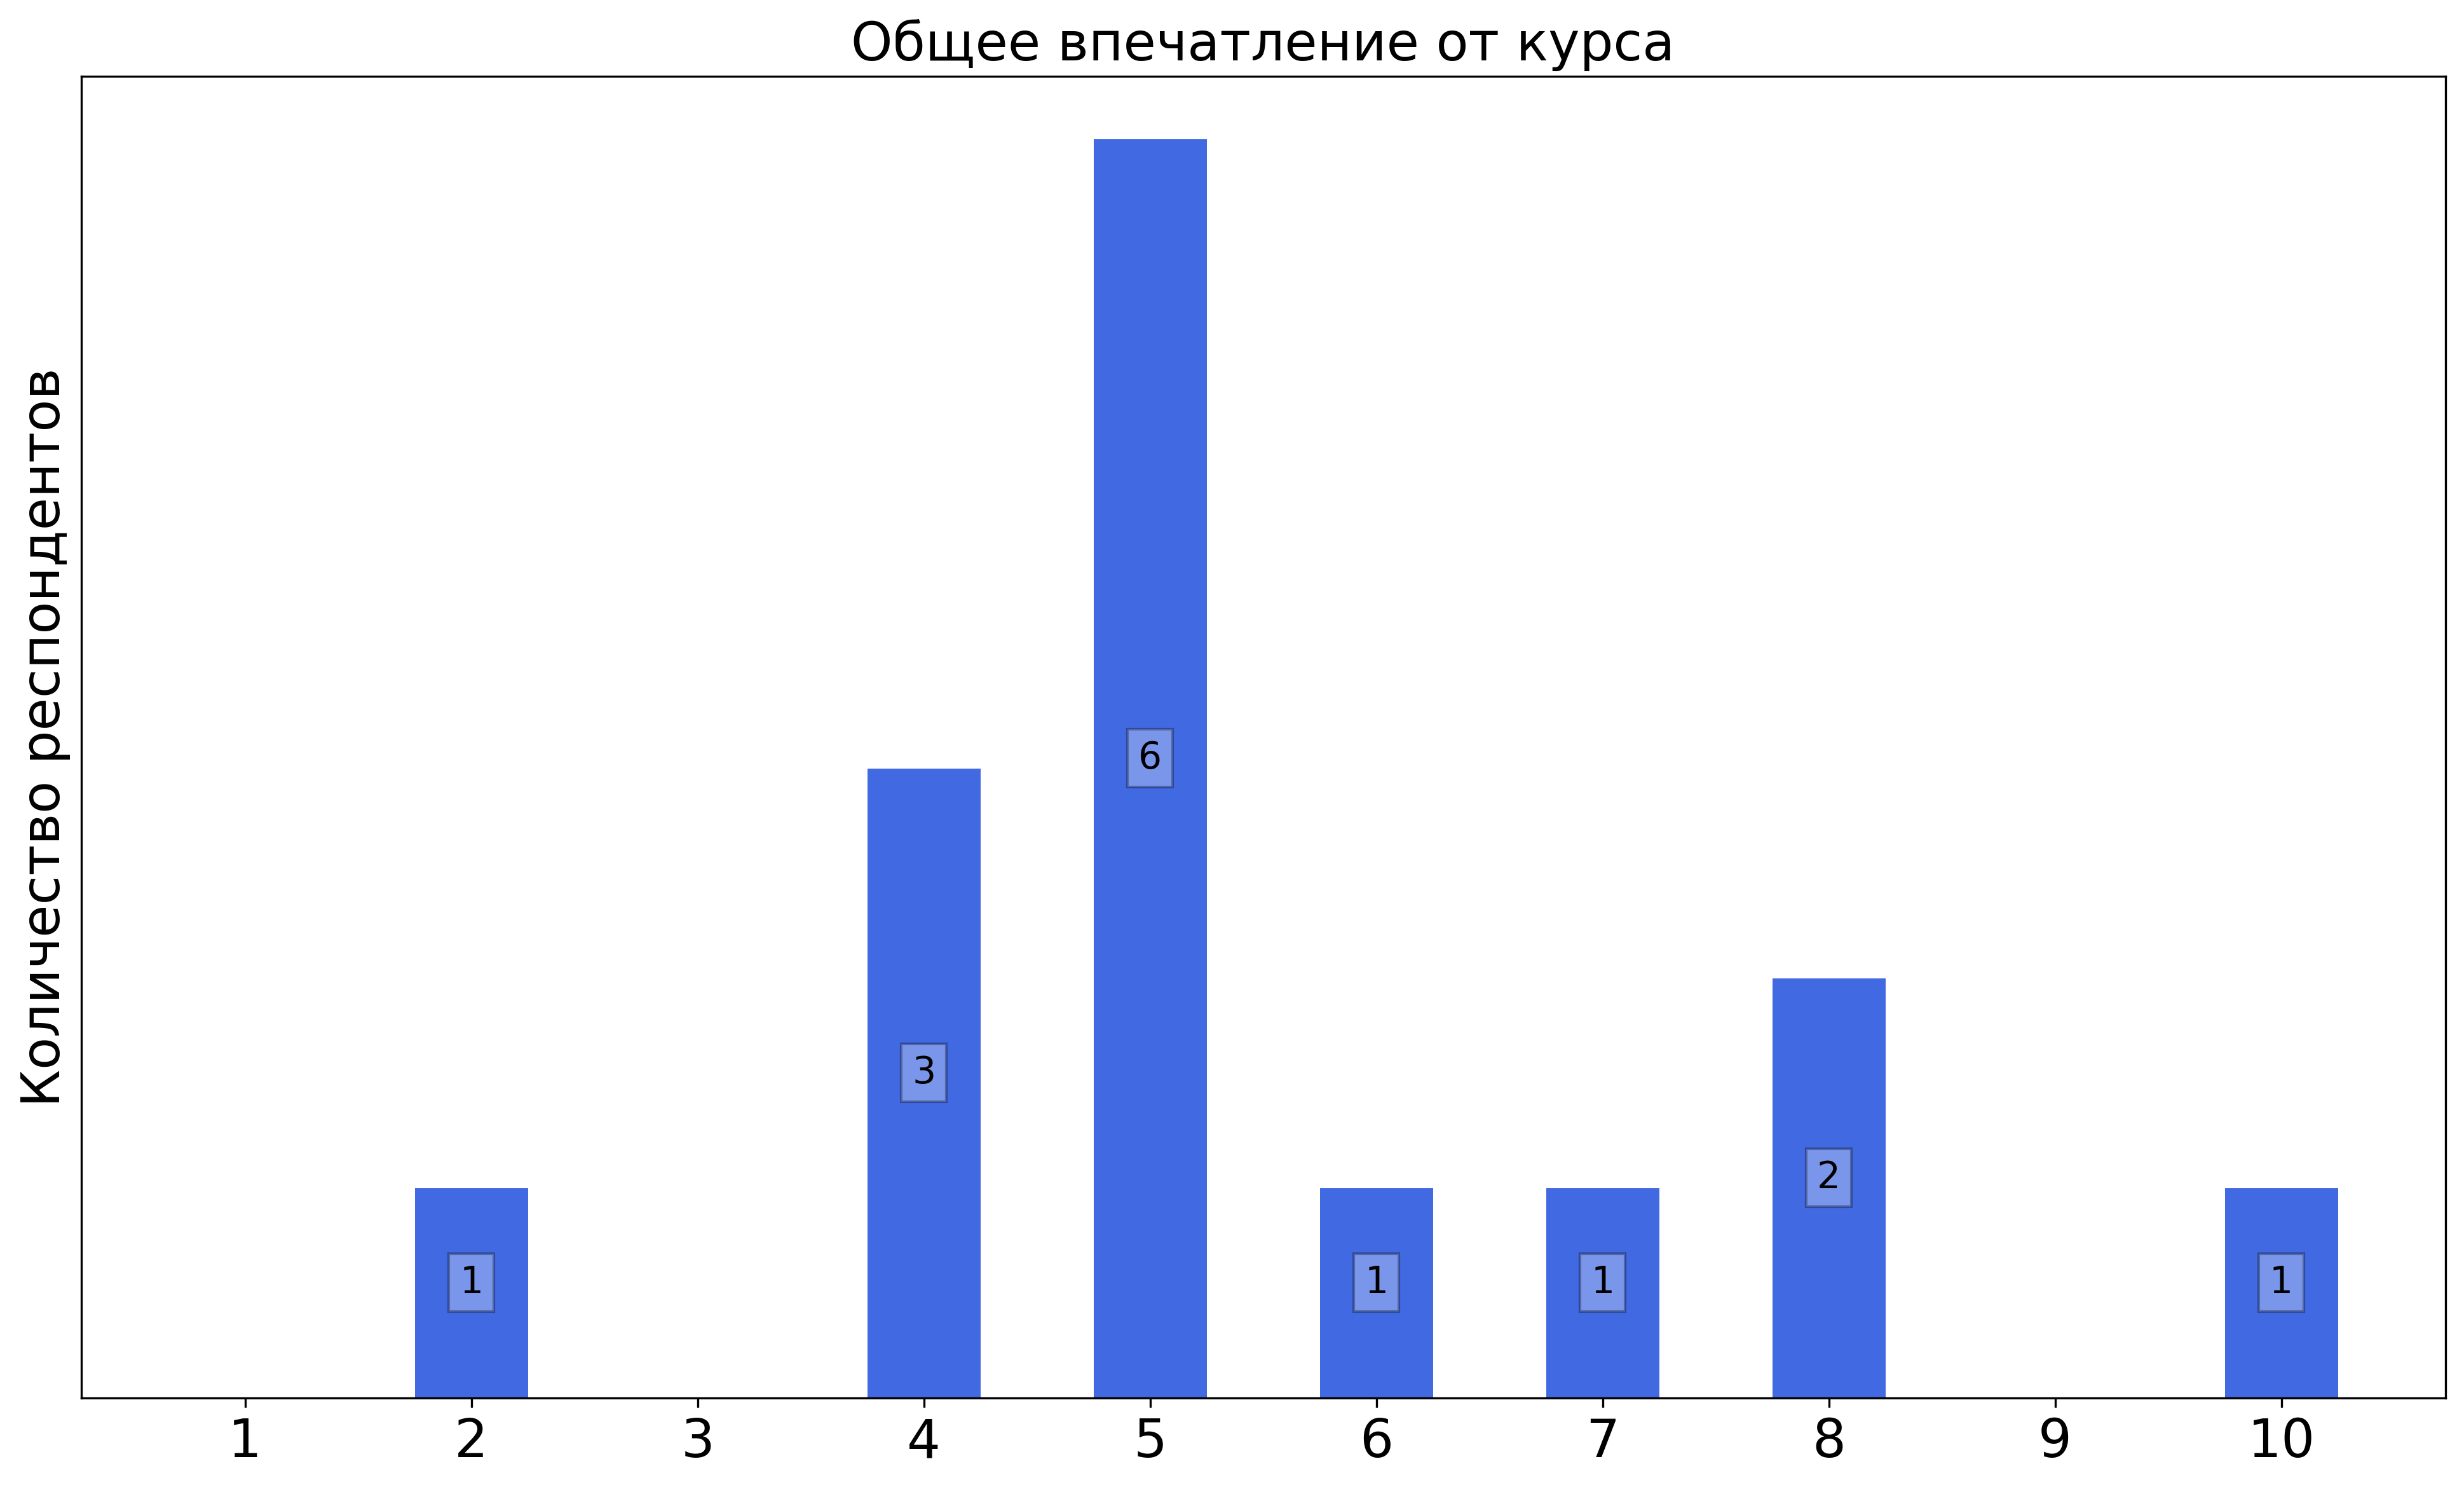
\includegraphics[width=\textwidth]{images/4 course/Введение в распараллеливание алгоритмов и программ/general-0.png}
			\end{subfigure}
		\end{figure}

	\subsubsection{Материалы, использумые респондентами при изучении курса}

		\begin{figure}[H]
			\centering
			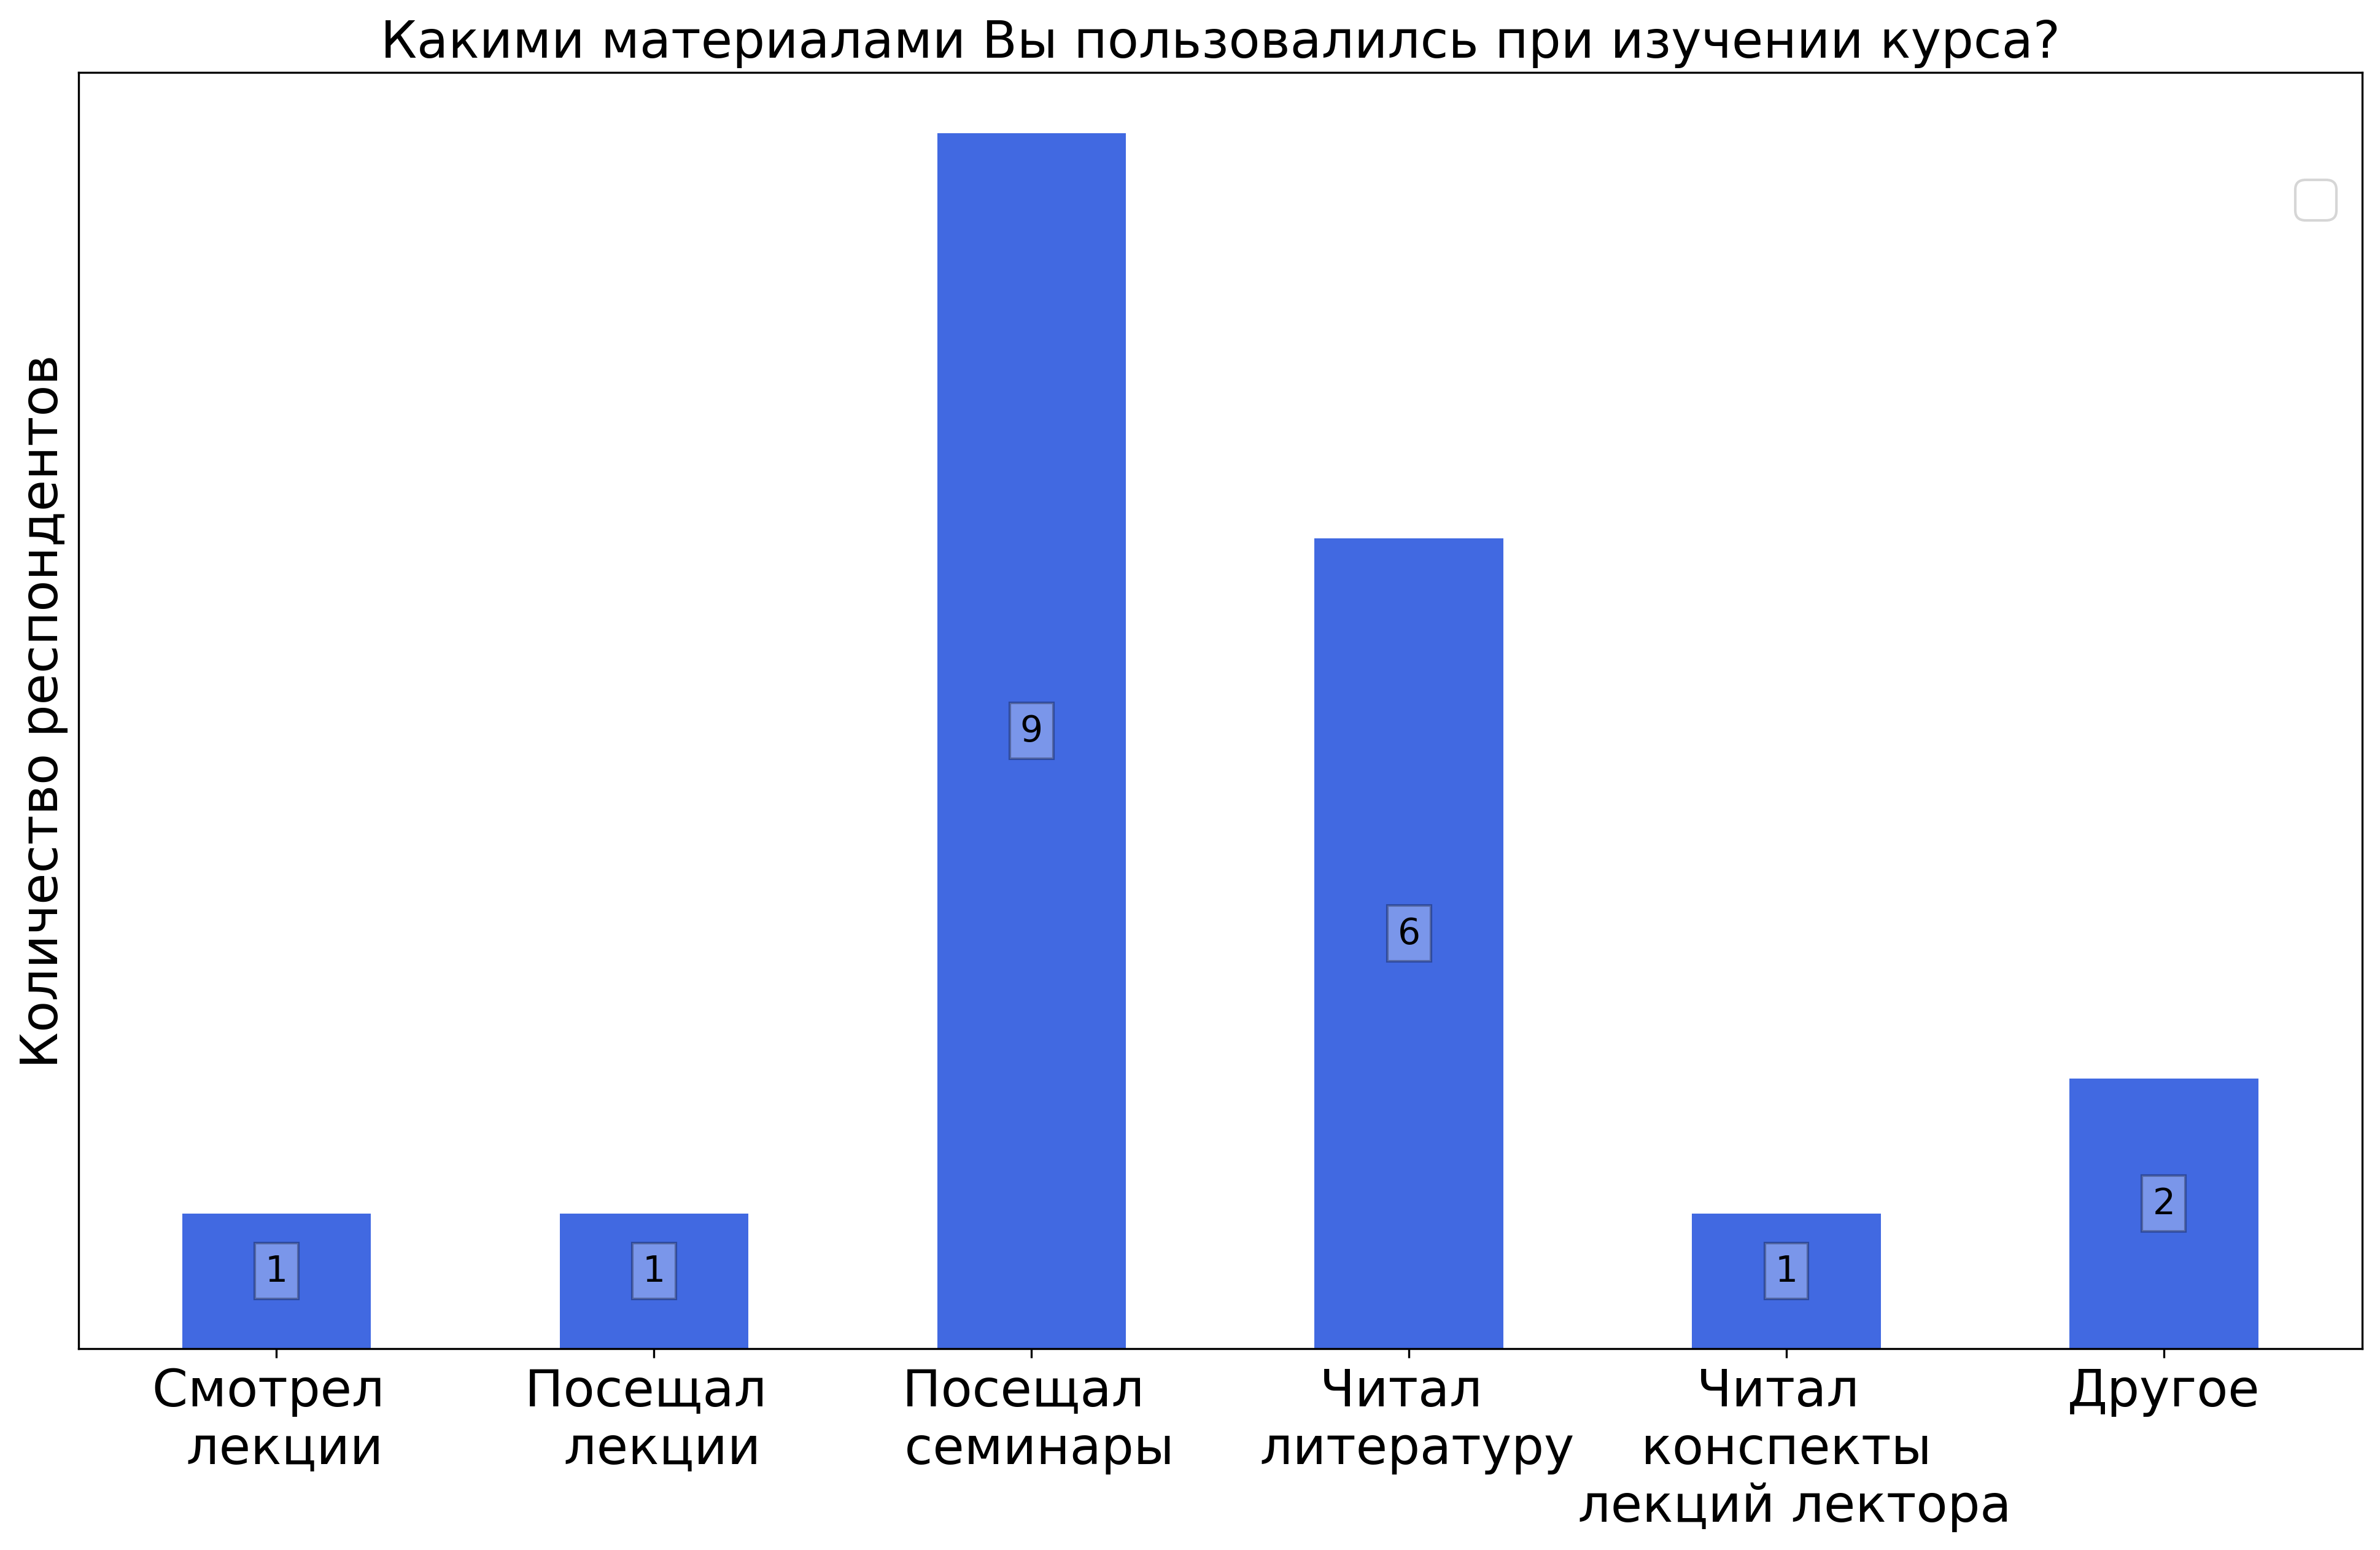
\includegraphics[width = 0.45\textwidth]{images/4 course/Введение в распараллеливание алгоритмов и программ/materials.png}
		\end{figure}

		\textit{В качестве других источников информации студенты указали:} 
		\begin{itemize}
			\item презентации семинариста.
		\end{itemize}

	\subsubsection{Отзыв студентов о лекциях. Лектор: Карпов В.Е.}

		\begin{figure}[H]
			\centering
            \begin{subfigure}[b]{0.45\textwidth}
				\centering
				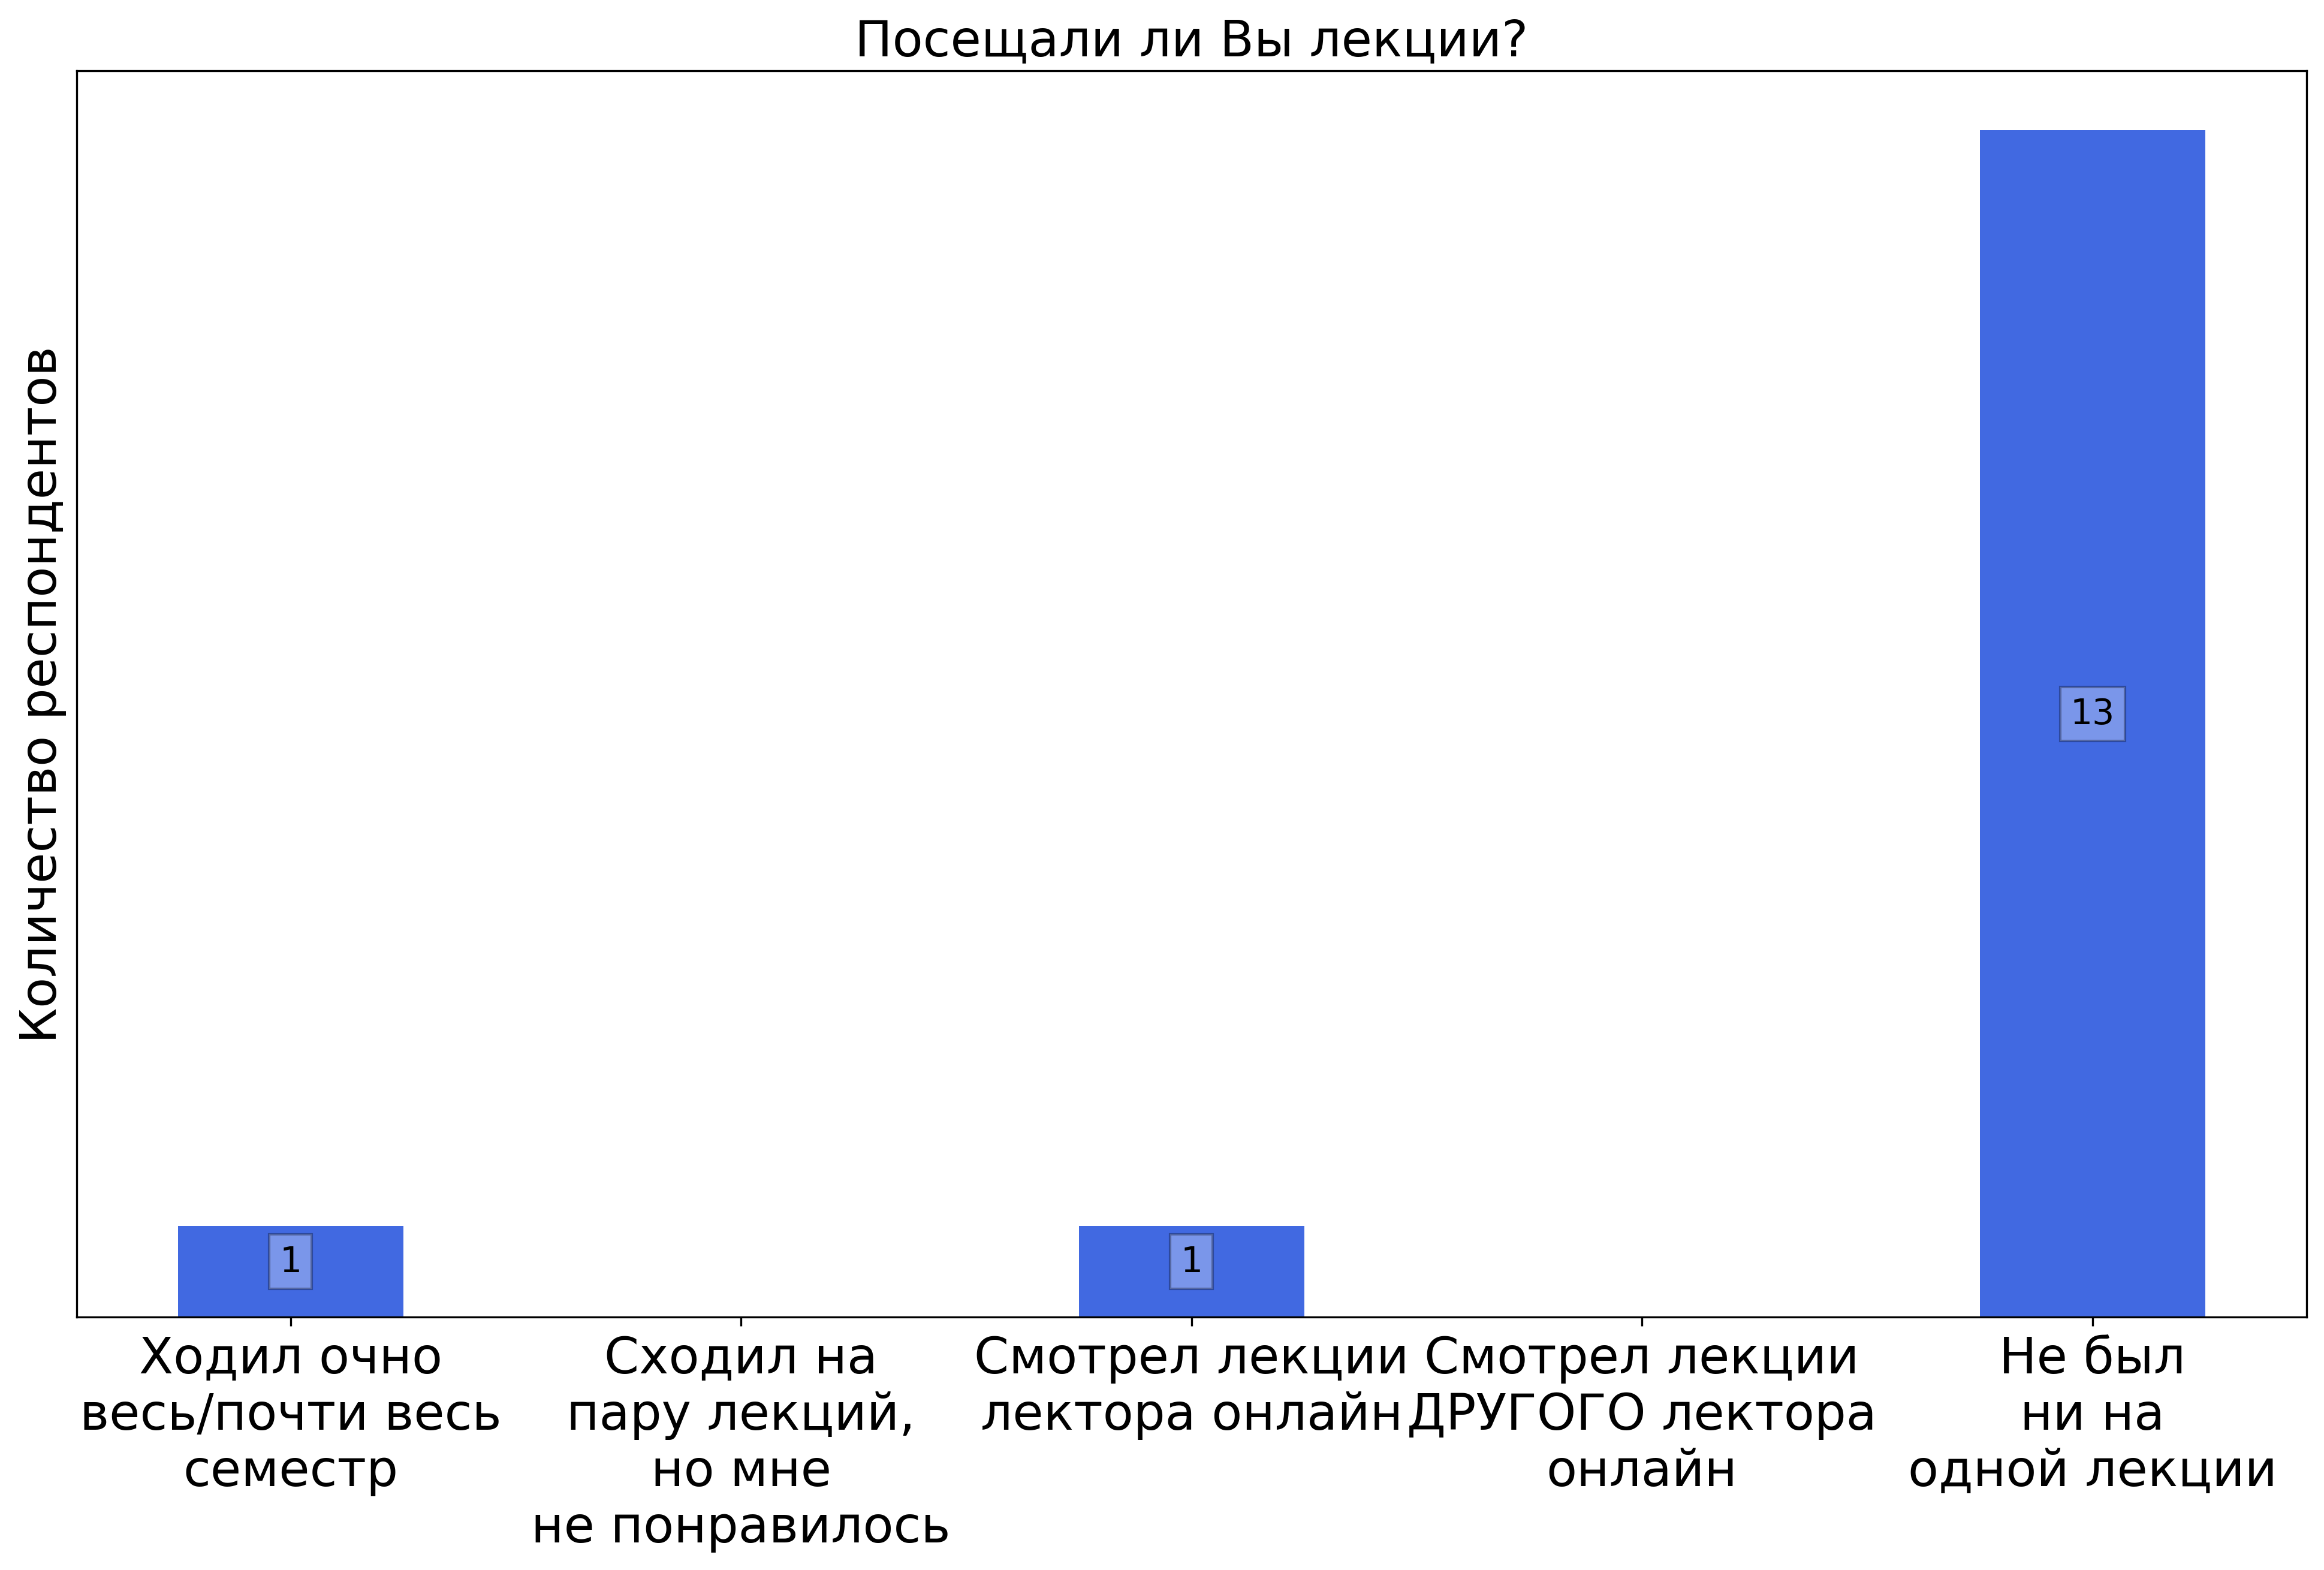
\includegraphics[width=\textwidth]{images/4 course/Введение в распараллеливание алгоритмов и программ/lecturer-questions-Карпов В.Е.-0.png}
			\end{subfigure}
			\begin{subfigure}[b]{0.45\textwidth}
				\centering
				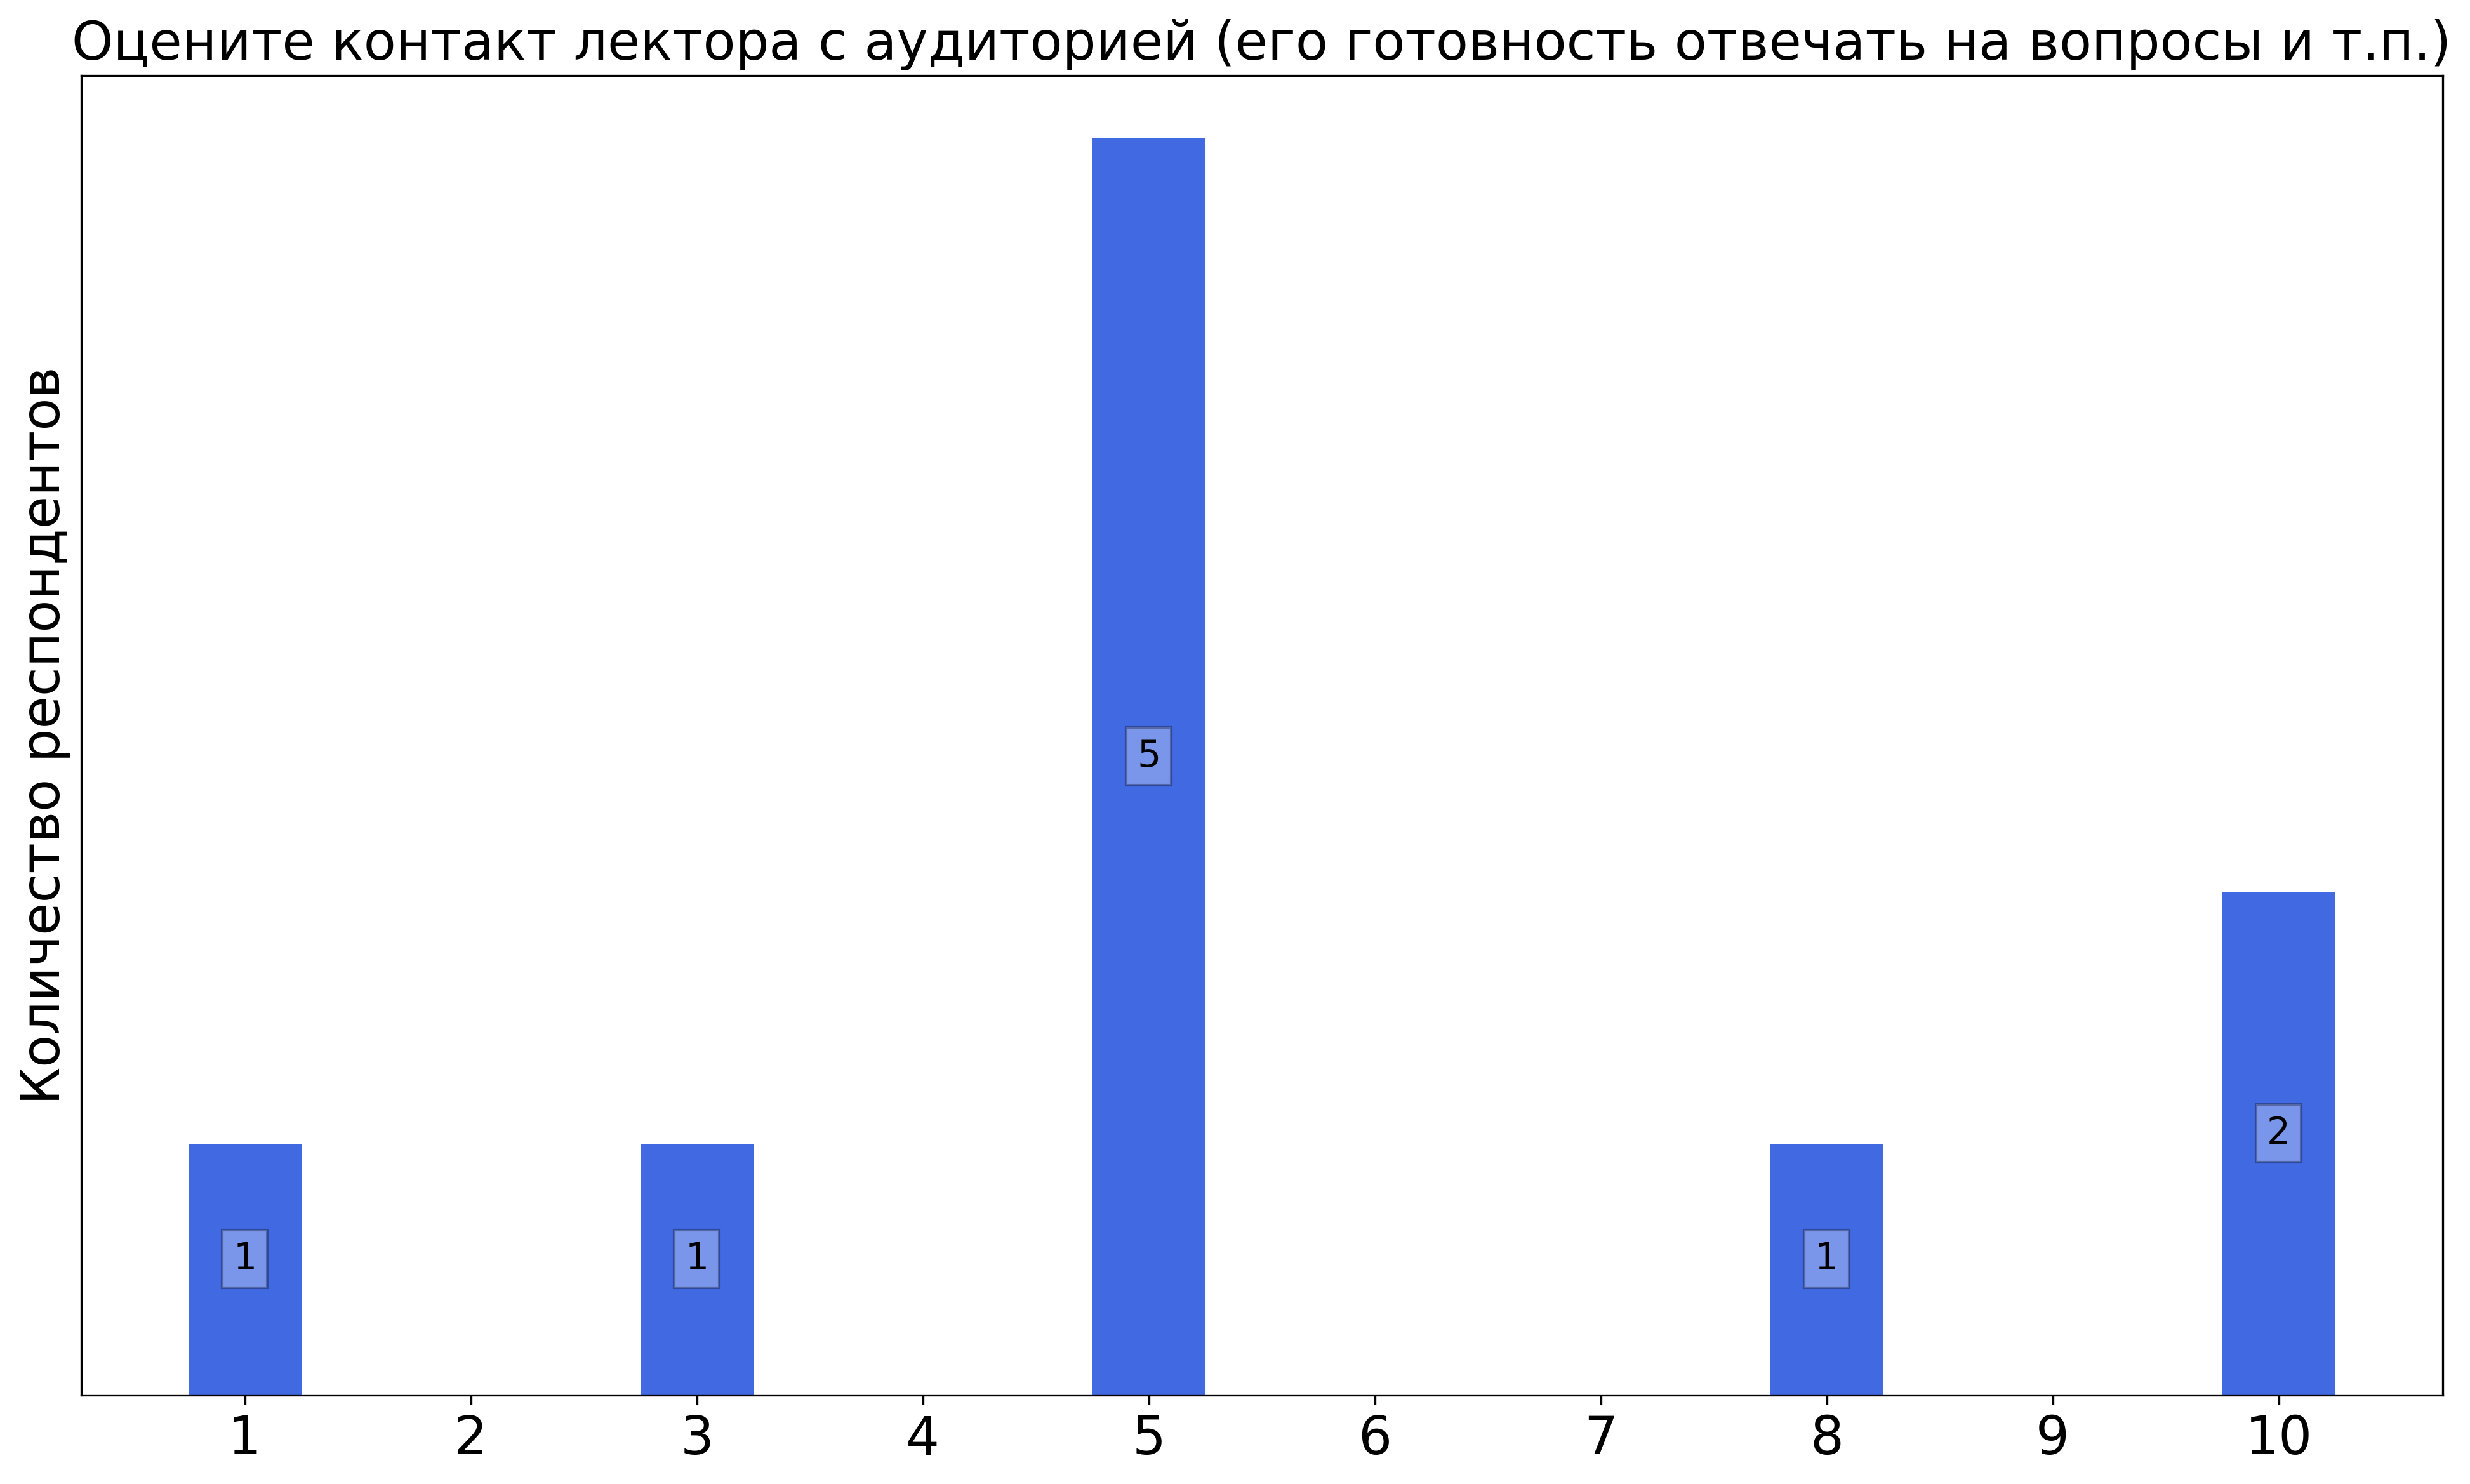
\includegraphics[width=\textwidth]{images/4 course/Введение в распараллеливание алгоритмов и программ/lecturer-marks-Карпов В.Е.-0.png}
			\end{subfigure}
			\begin{subfigure}[b]{0.45\textwidth}
				\centering
				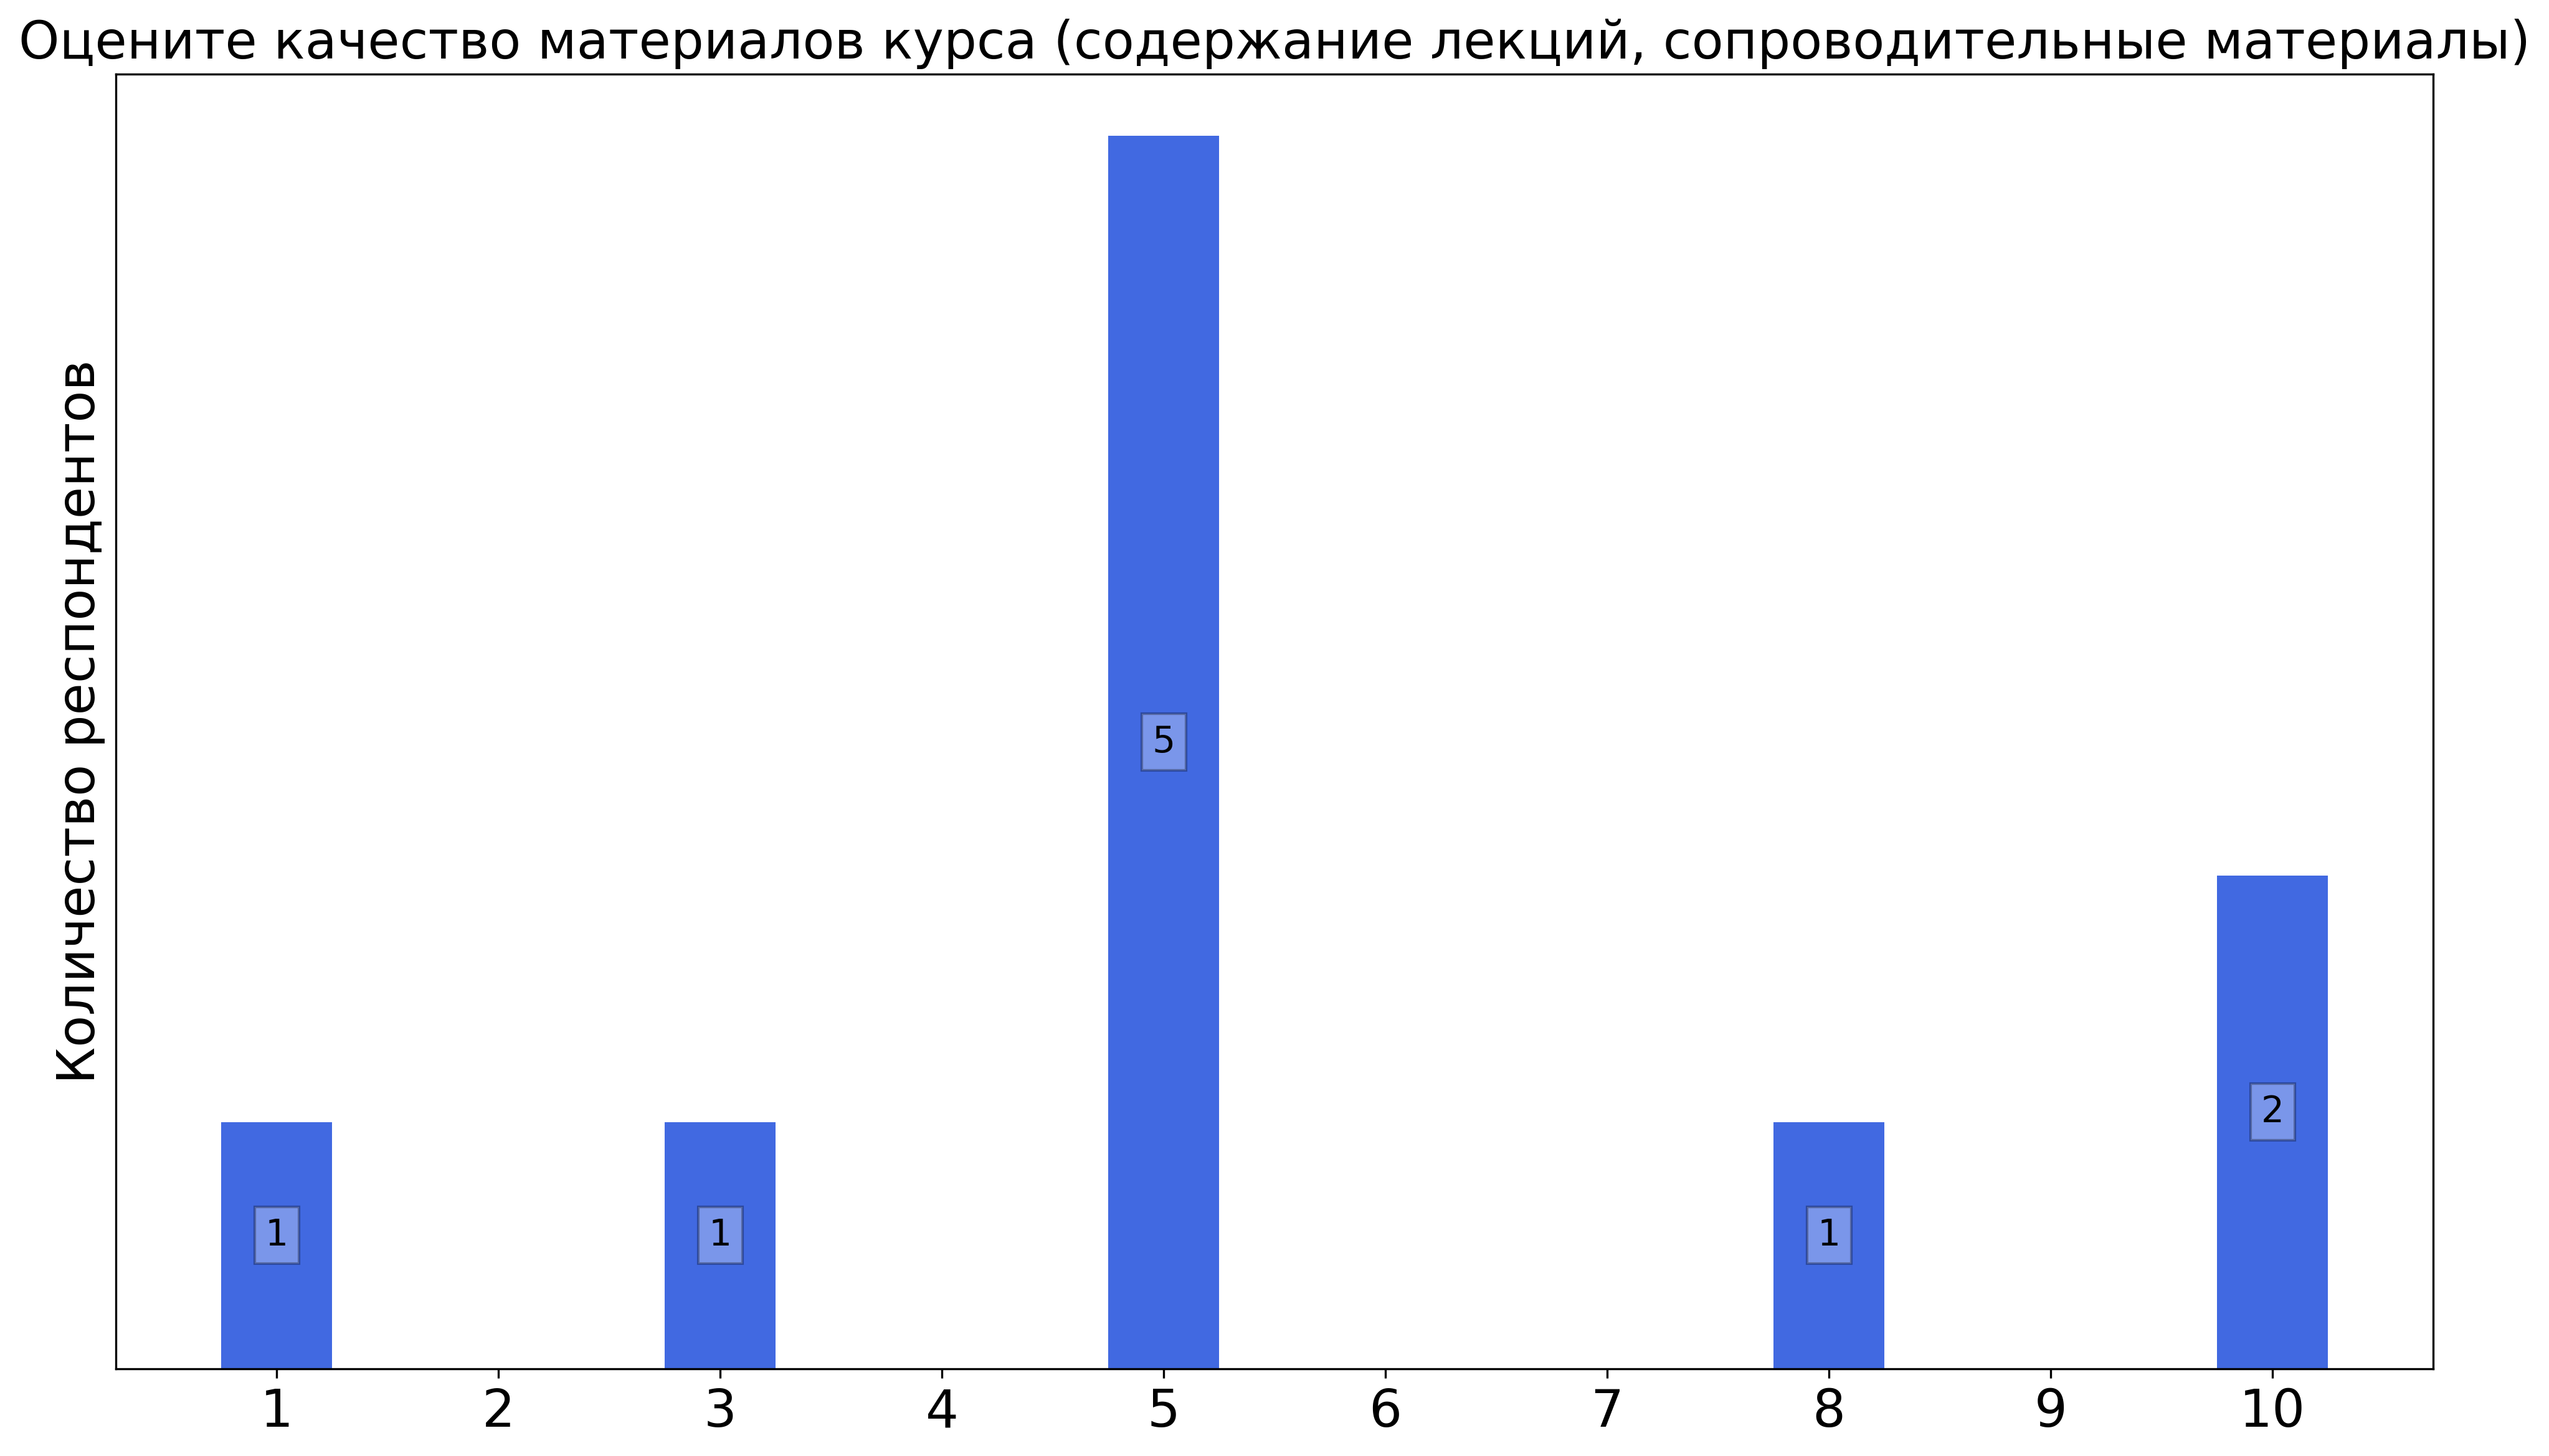
\includegraphics[width=\textwidth]{images/4 course/Введение в распараллеливание алгоритмов и программ/lecturer-marks-Карпов В.Е.-1.png}
			\end{subfigure}
			\begin{subfigure}[b]{0.45\textwidth}
				\centering
				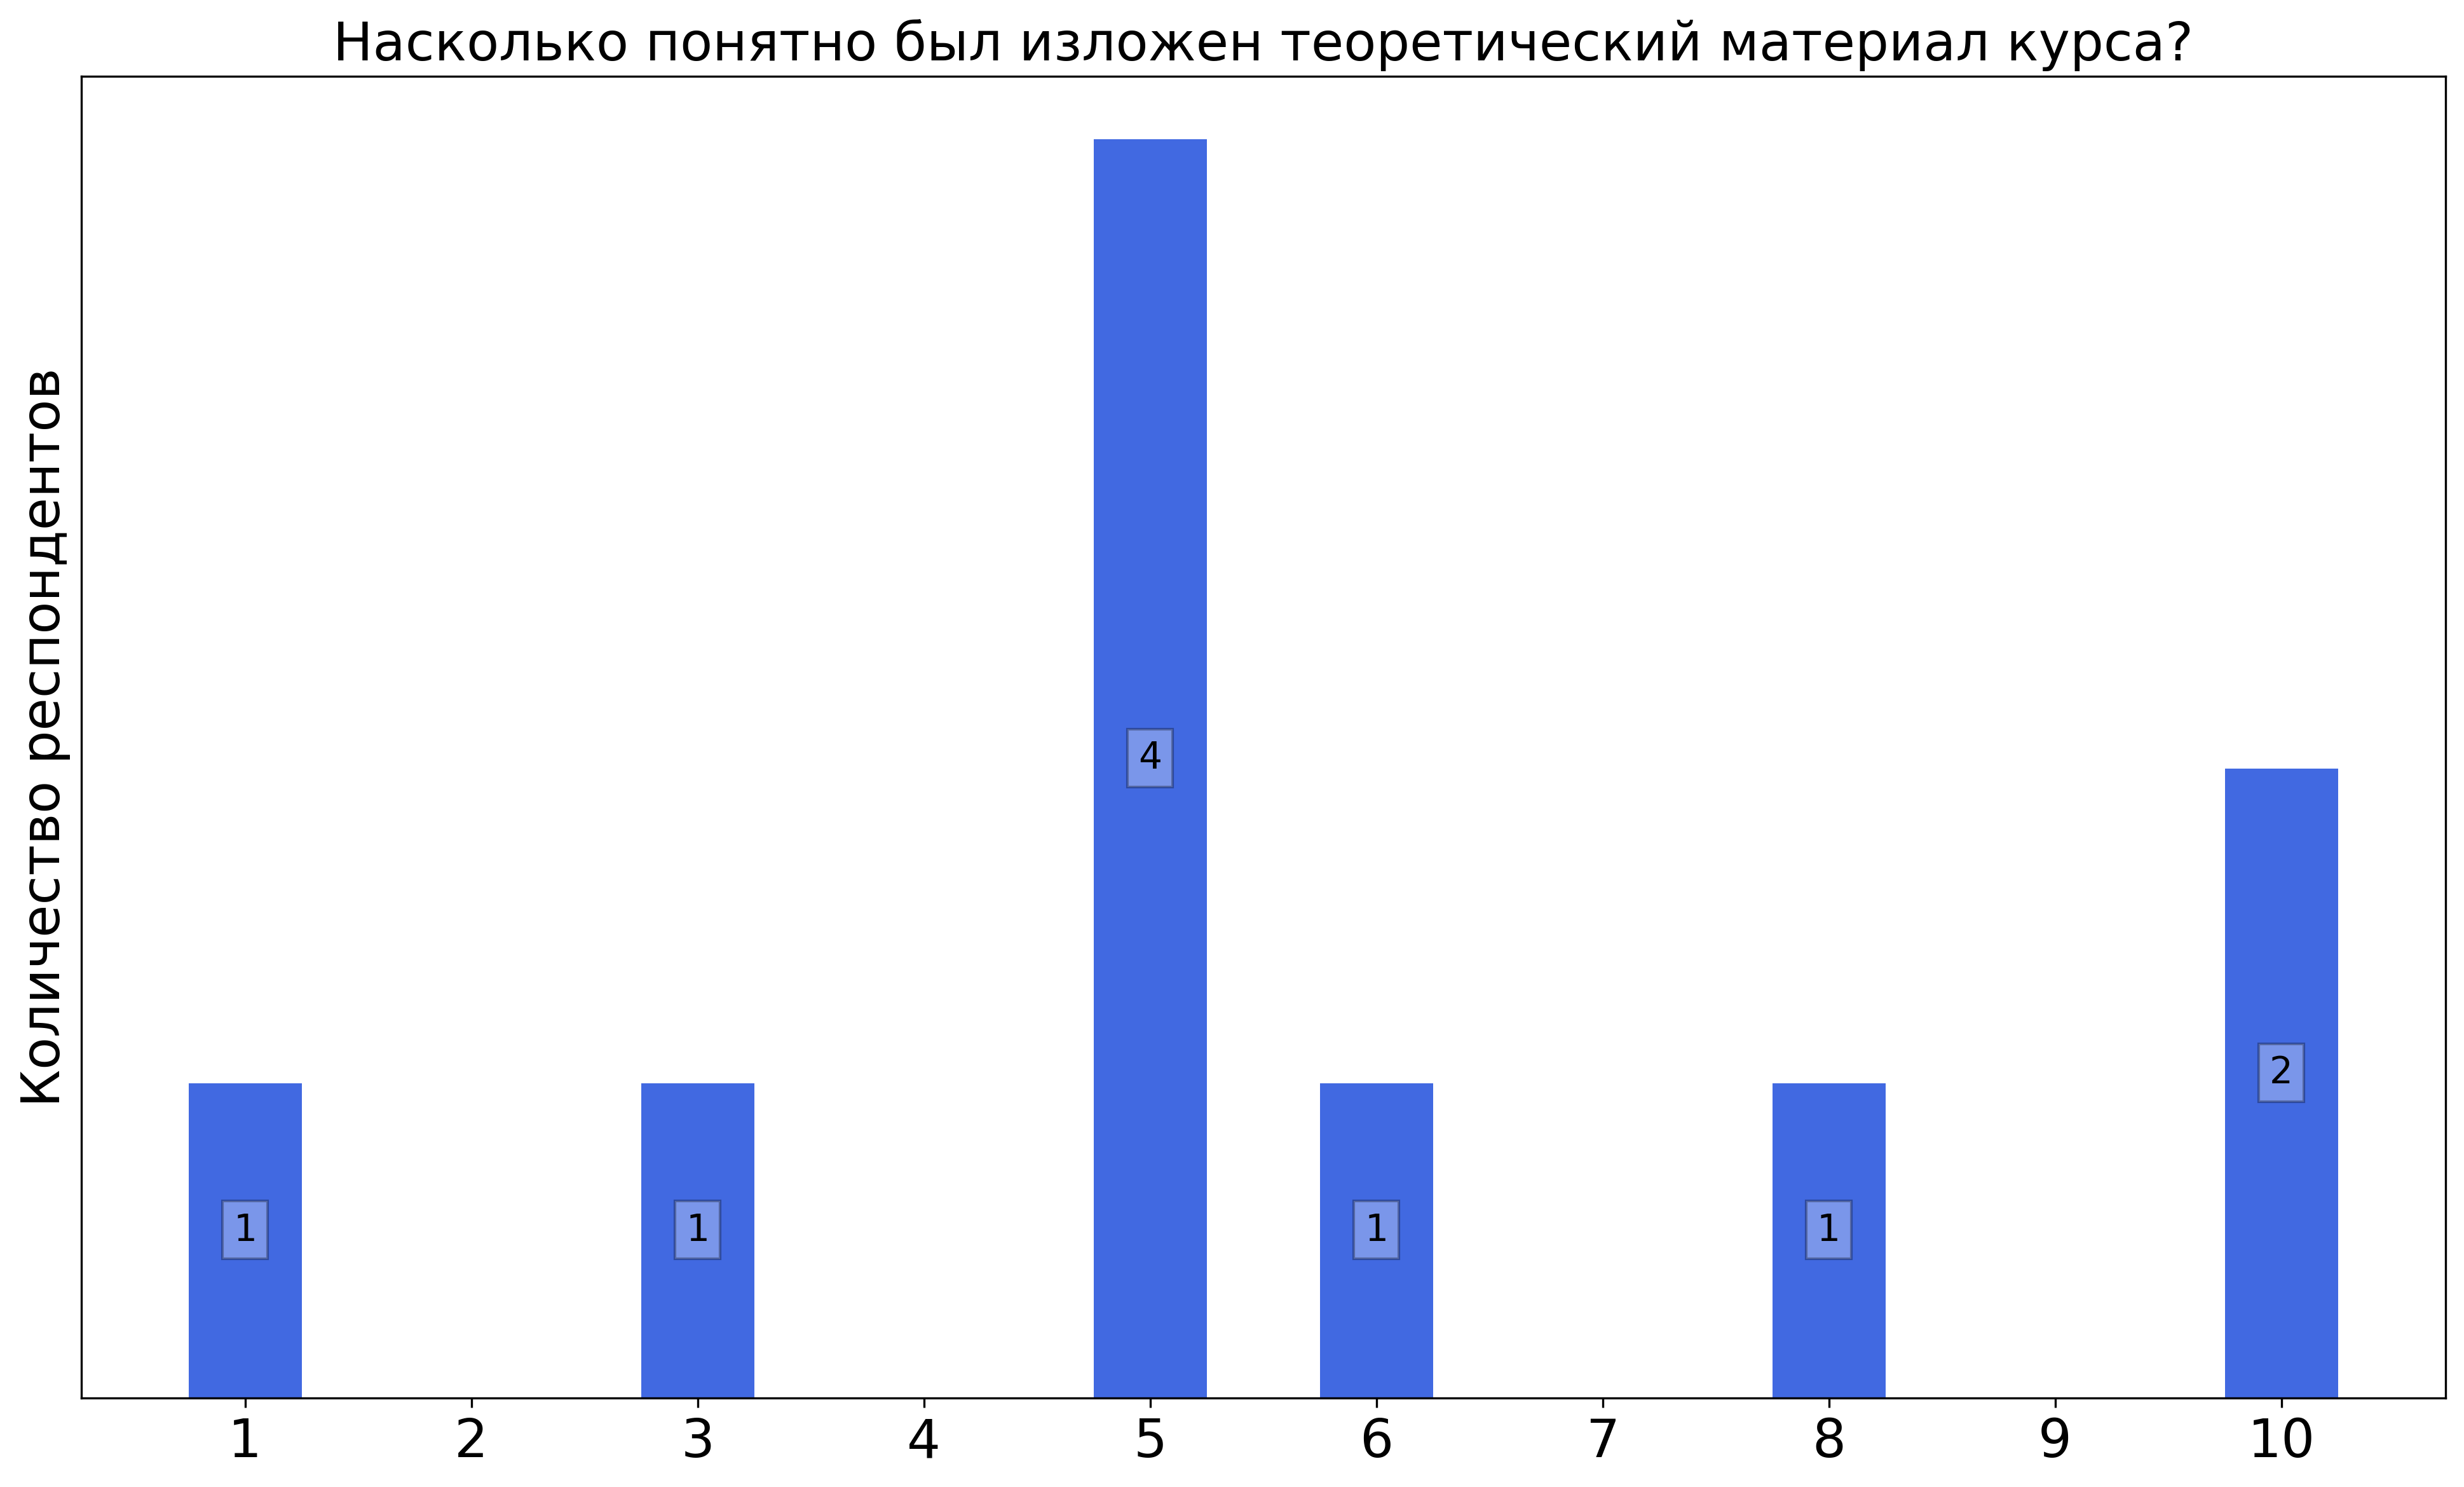
\includegraphics[width=\textwidth]{images/4 course/Введение в распараллеливание алгоритмов и программ/lecturer-marks-Карпов В.Е.-2.png}
			\end{subfigure}	
			\begin{subfigure}[b]{0.45\textwidth}
				\centering
				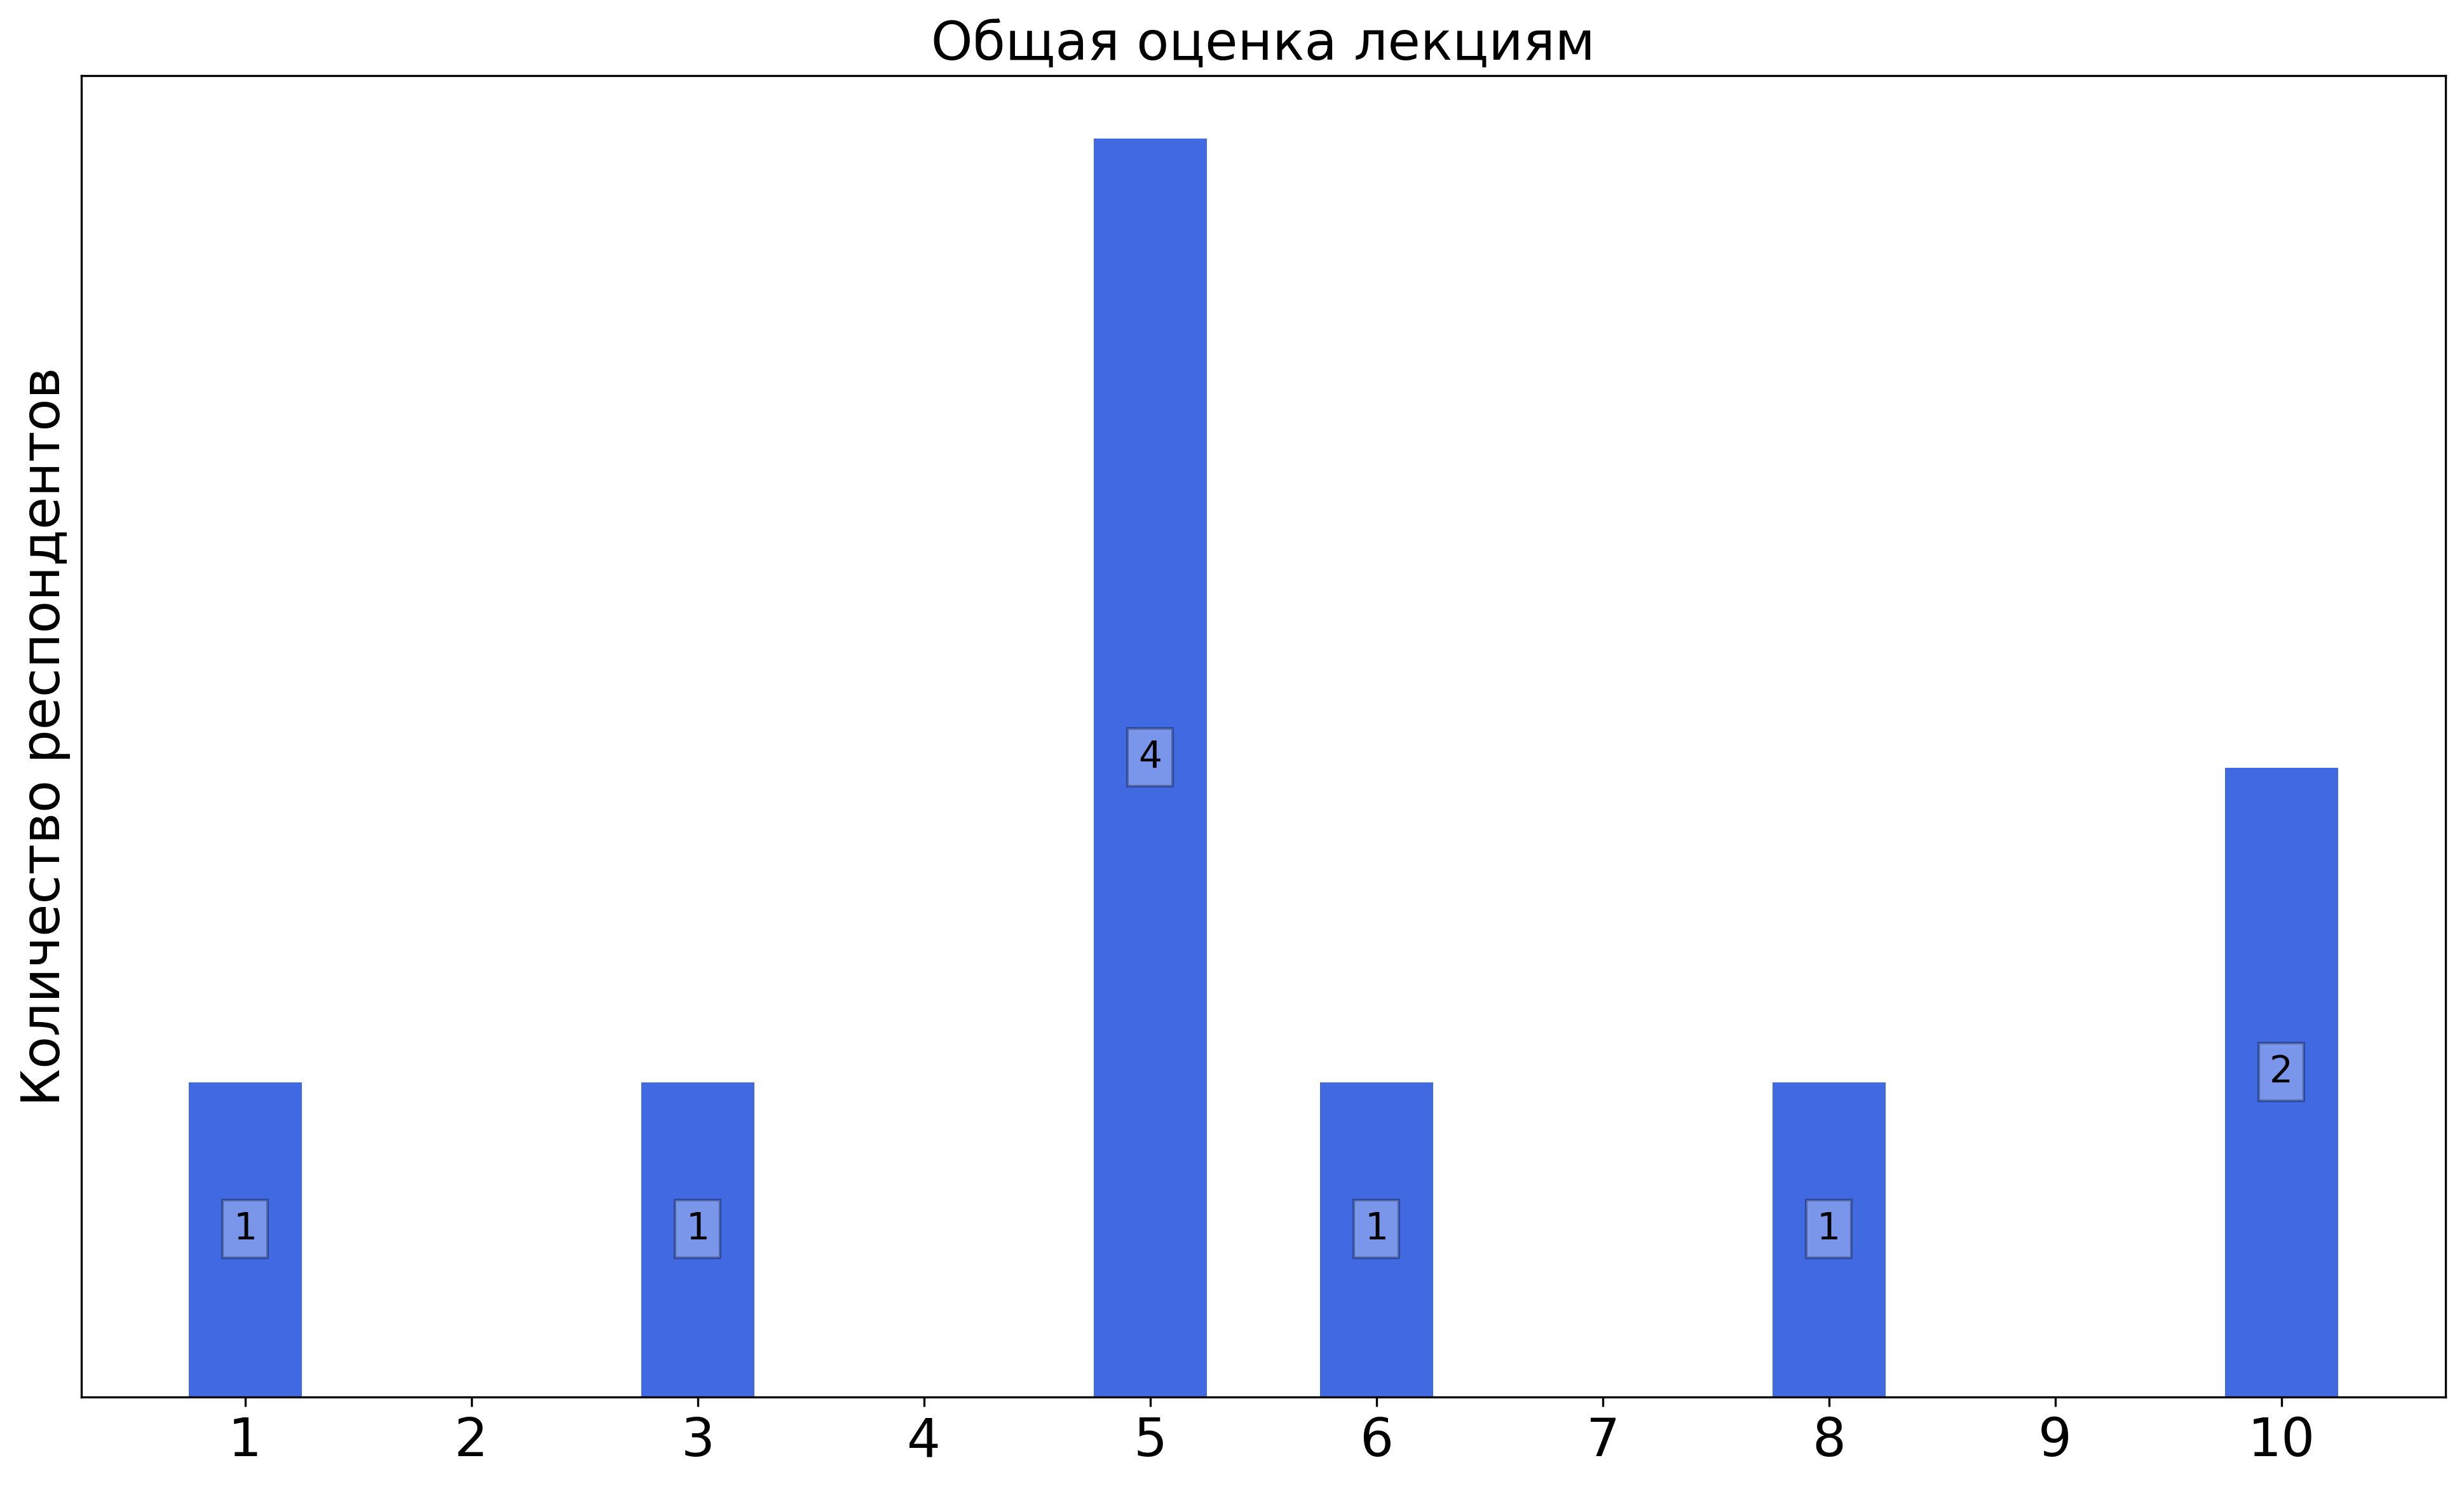
\includegraphics[width=\textwidth]{images/4 course/Введение в распараллеливание алгоритмов и программ/lecturer-marks-Карпов В.Е.-3.png}
			\end{subfigure}
			\caption{Оценки респондентов о качестве преподавания лекций по курсу <<Введение в распараллеливание алгоритмов и программ>>}
		\end{figure}

		\textbf{Комментарии студентов о лекциях\protect\footnote{сохранены оригинальные орфография и пунктуация}}
            \begin{commentbox} 
                Мне не хватило времени посещать лекции но то что я видела на семинарах касательно программы курса сформировало мое мнение. Я считаю курс несколько устарел по технологиям, мне бы хотелось видеть более востребованные фреймворки чем openmp/mpi. Мне не было актуально так же взаимодействие вычматов и парпроги (это вторая половина курса лекций этого семестра). Я не думаю что много кто на рт будет использовать распараллеливание в контексте вычислительной математики. 
            \end{commentbox} 
        
            \begin{commentbox} 
                Лекции абсолютно бесполезны 
            \end{commentbox}    

    
    \subsubsection{Отзыв студентов о семинарах. Семинарист: Лапушкин А.Г.}
		\begin{figure}[H]
			\centering
			\begin{subfigure}[b]{0.45\textwidth}
				\centering
				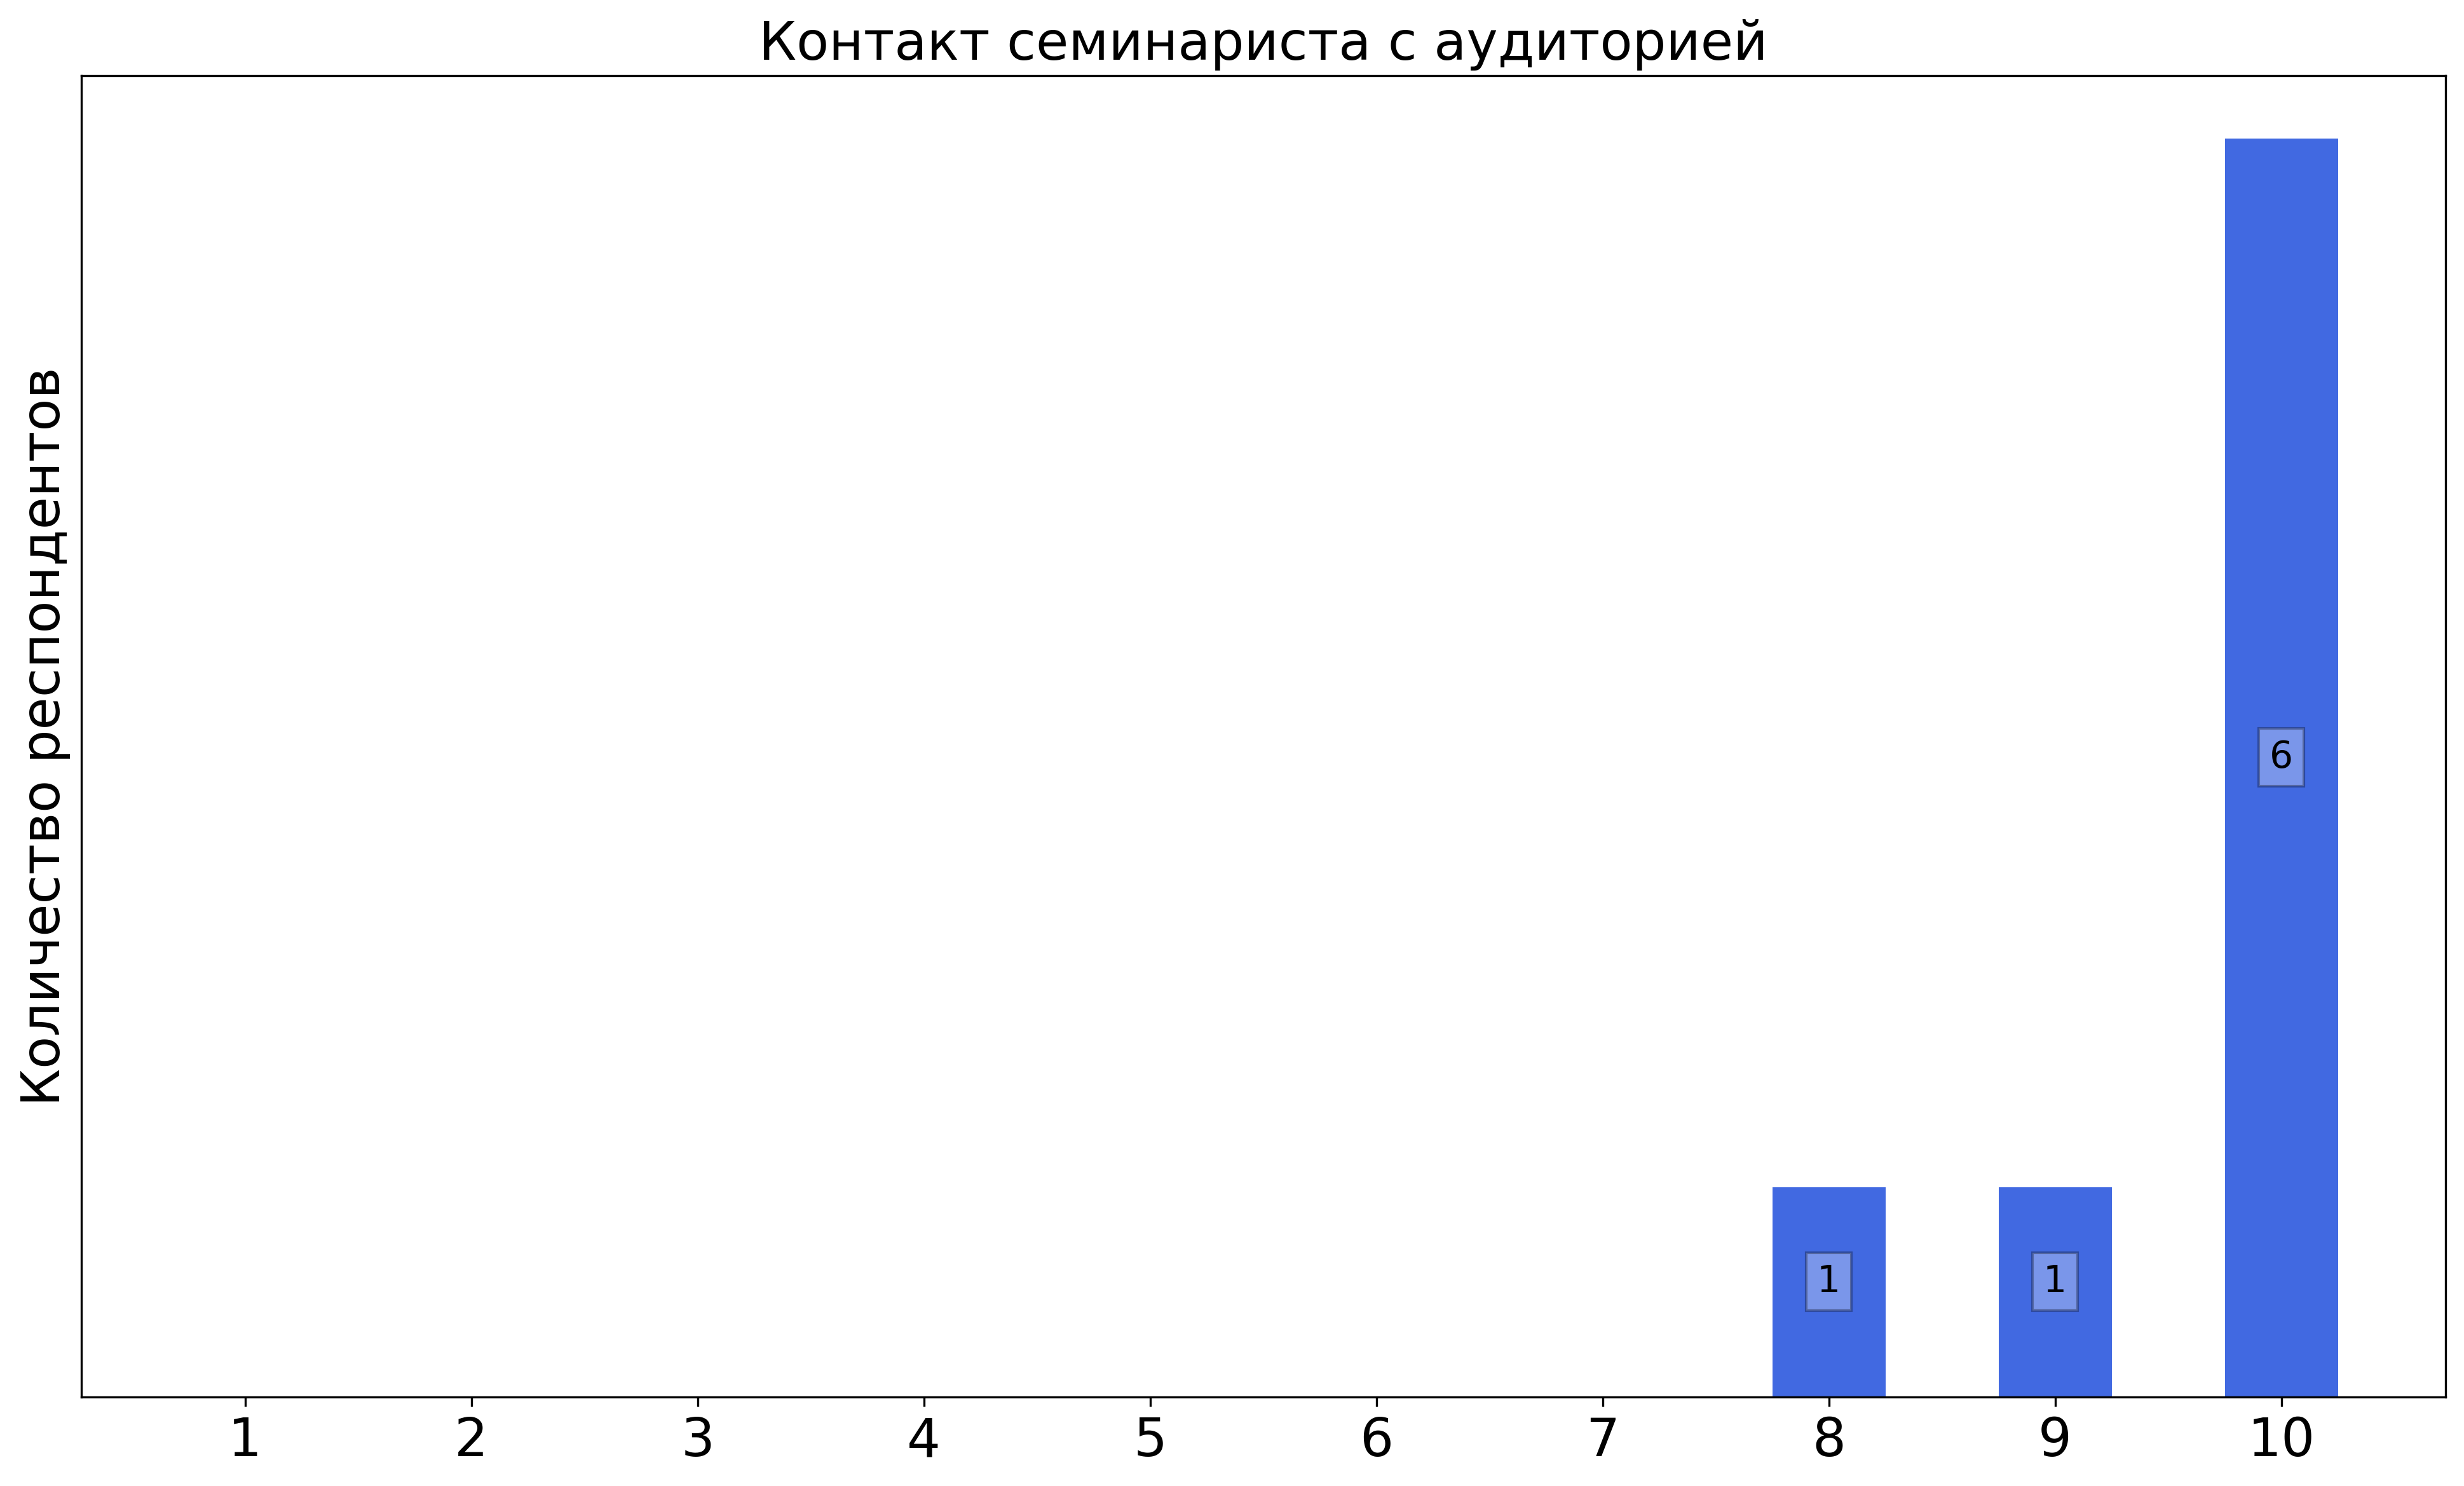
\includegraphics[width=\textwidth]{images/4 course/Введение в распараллеливание алгоритмов и программ/seminarists-marks-Лапушкин А.Г.-0.png}
			\end{subfigure}
			\begin{subfigure}[b]{0.45\textwidth}
				\centering
				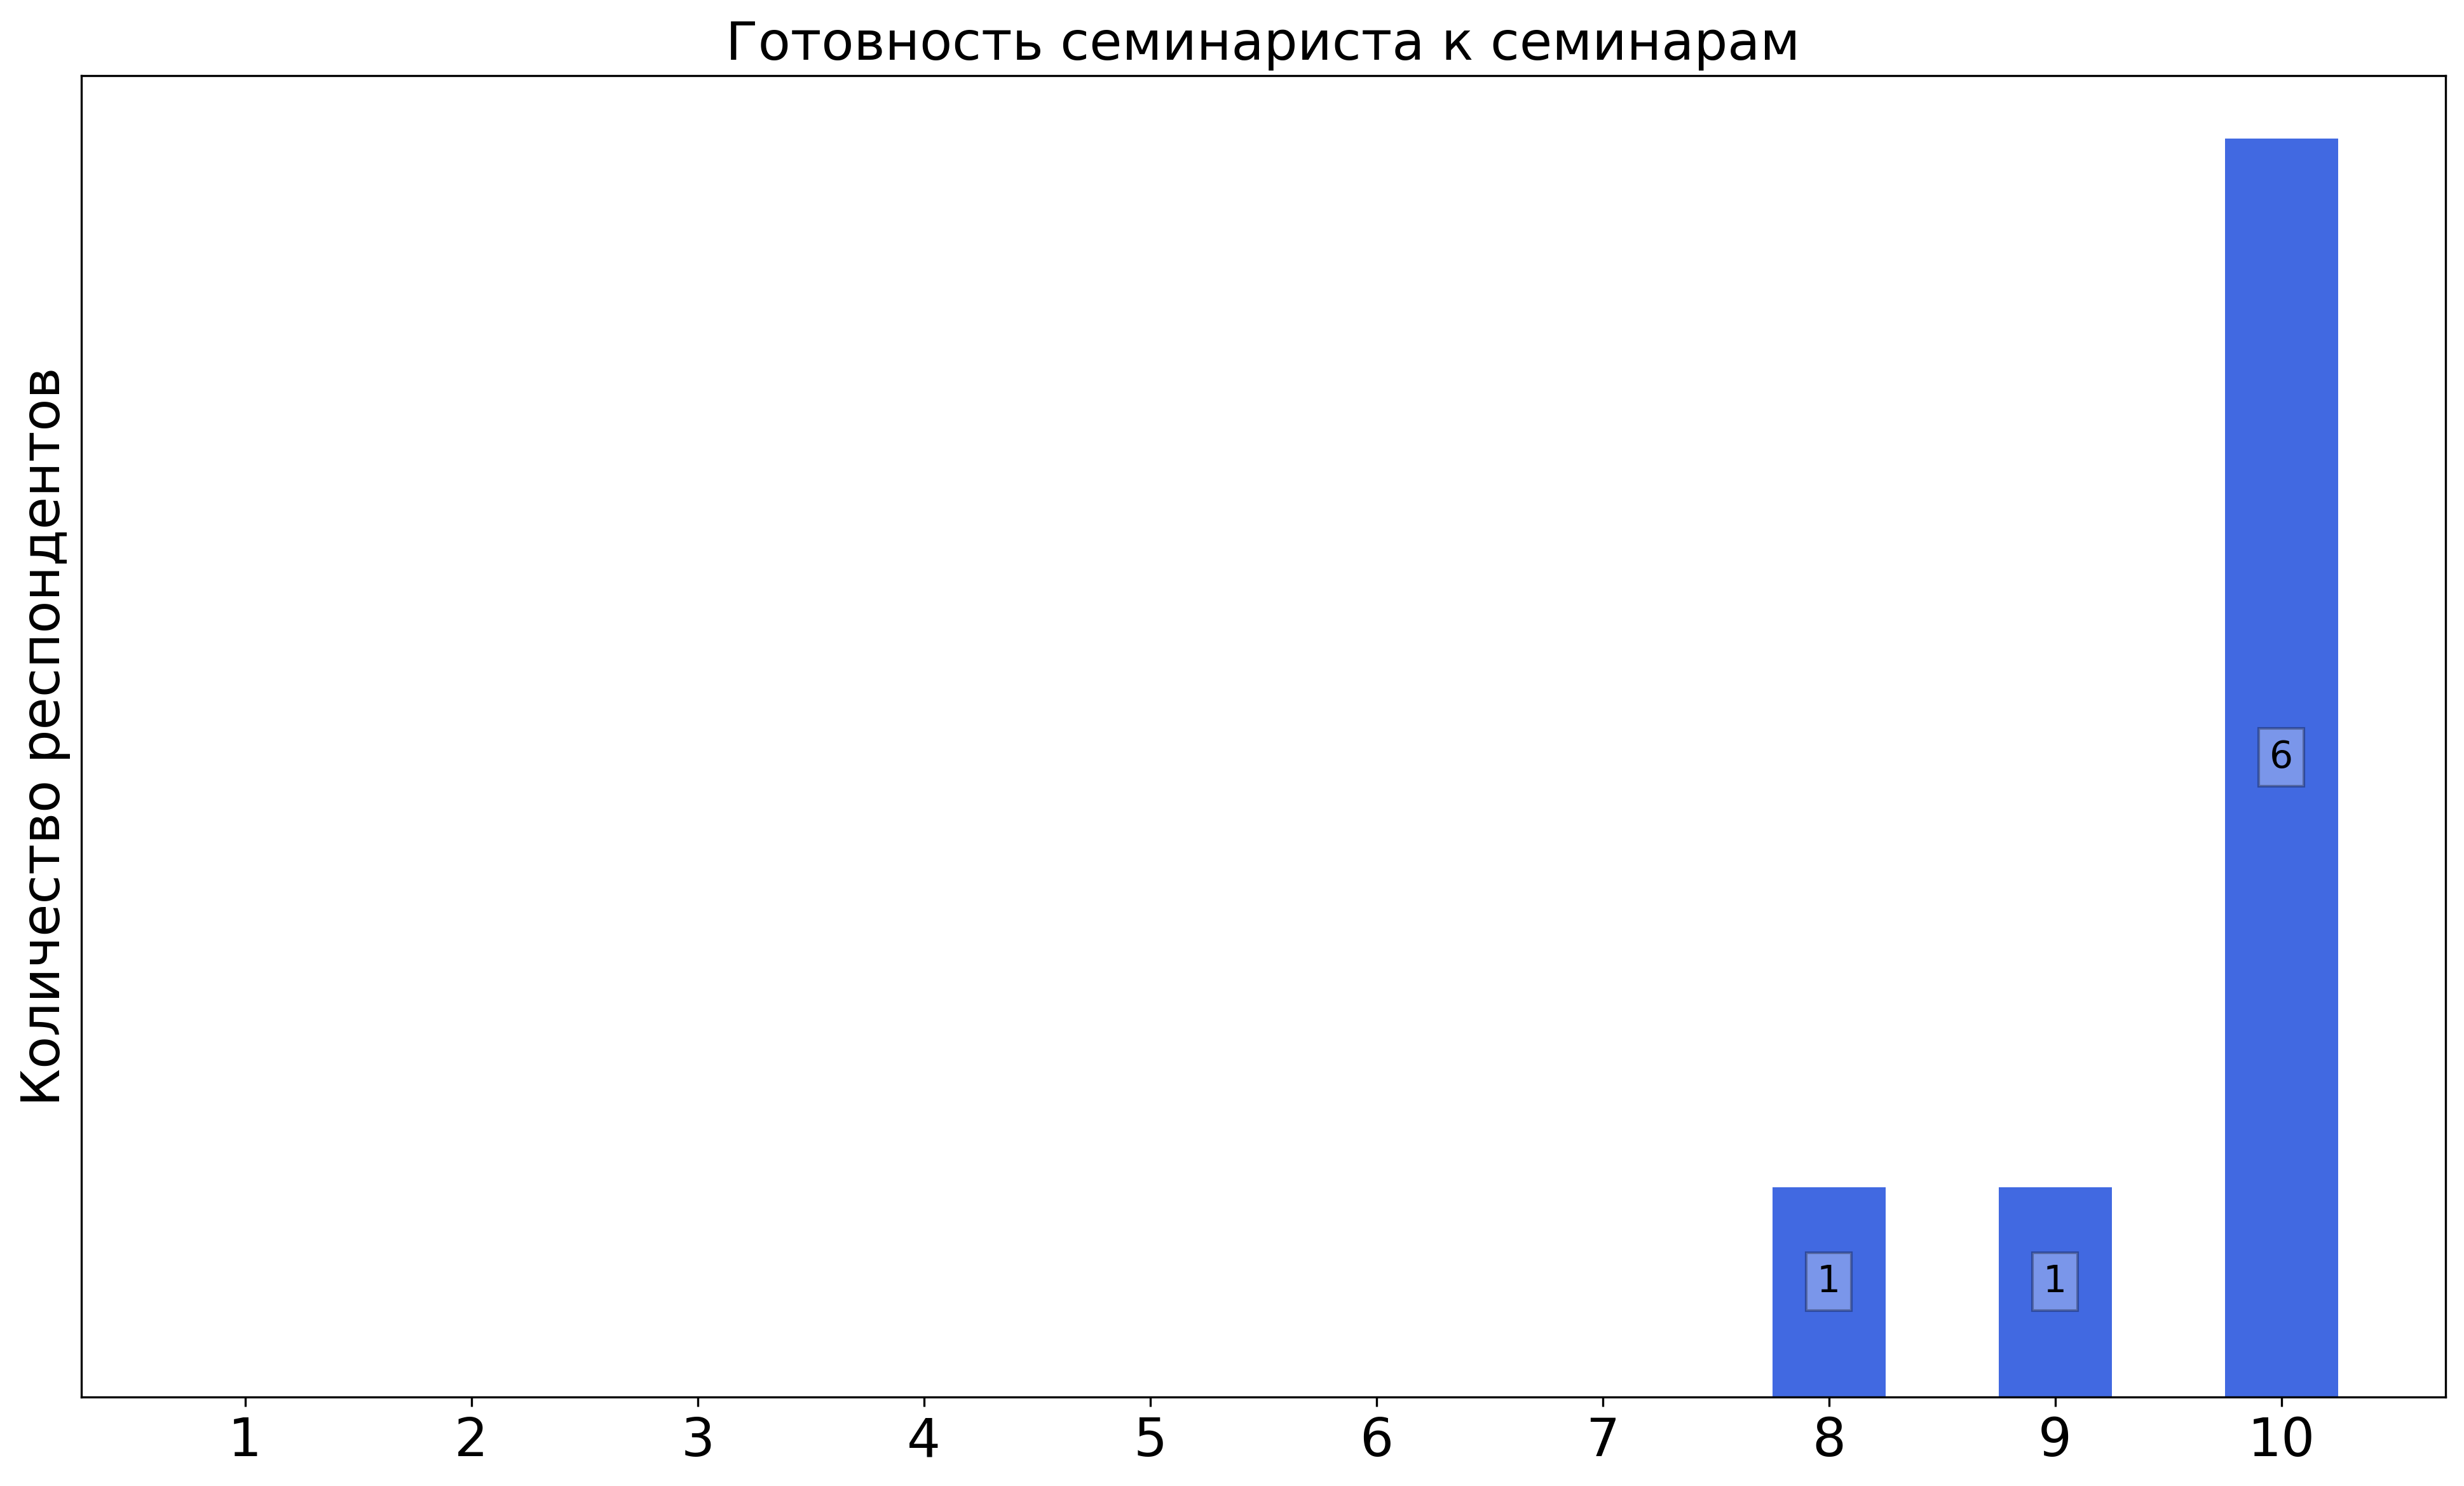
\includegraphics[width=\textwidth]{images/4 course/Введение в распараллеливание алгоритмов и программ/seminarists-marks-Лапушкин А.Г.-1.png}
			\end{subfigure}
			\begin{subfigure}[b]{0.45\textwidth}
				\centering
				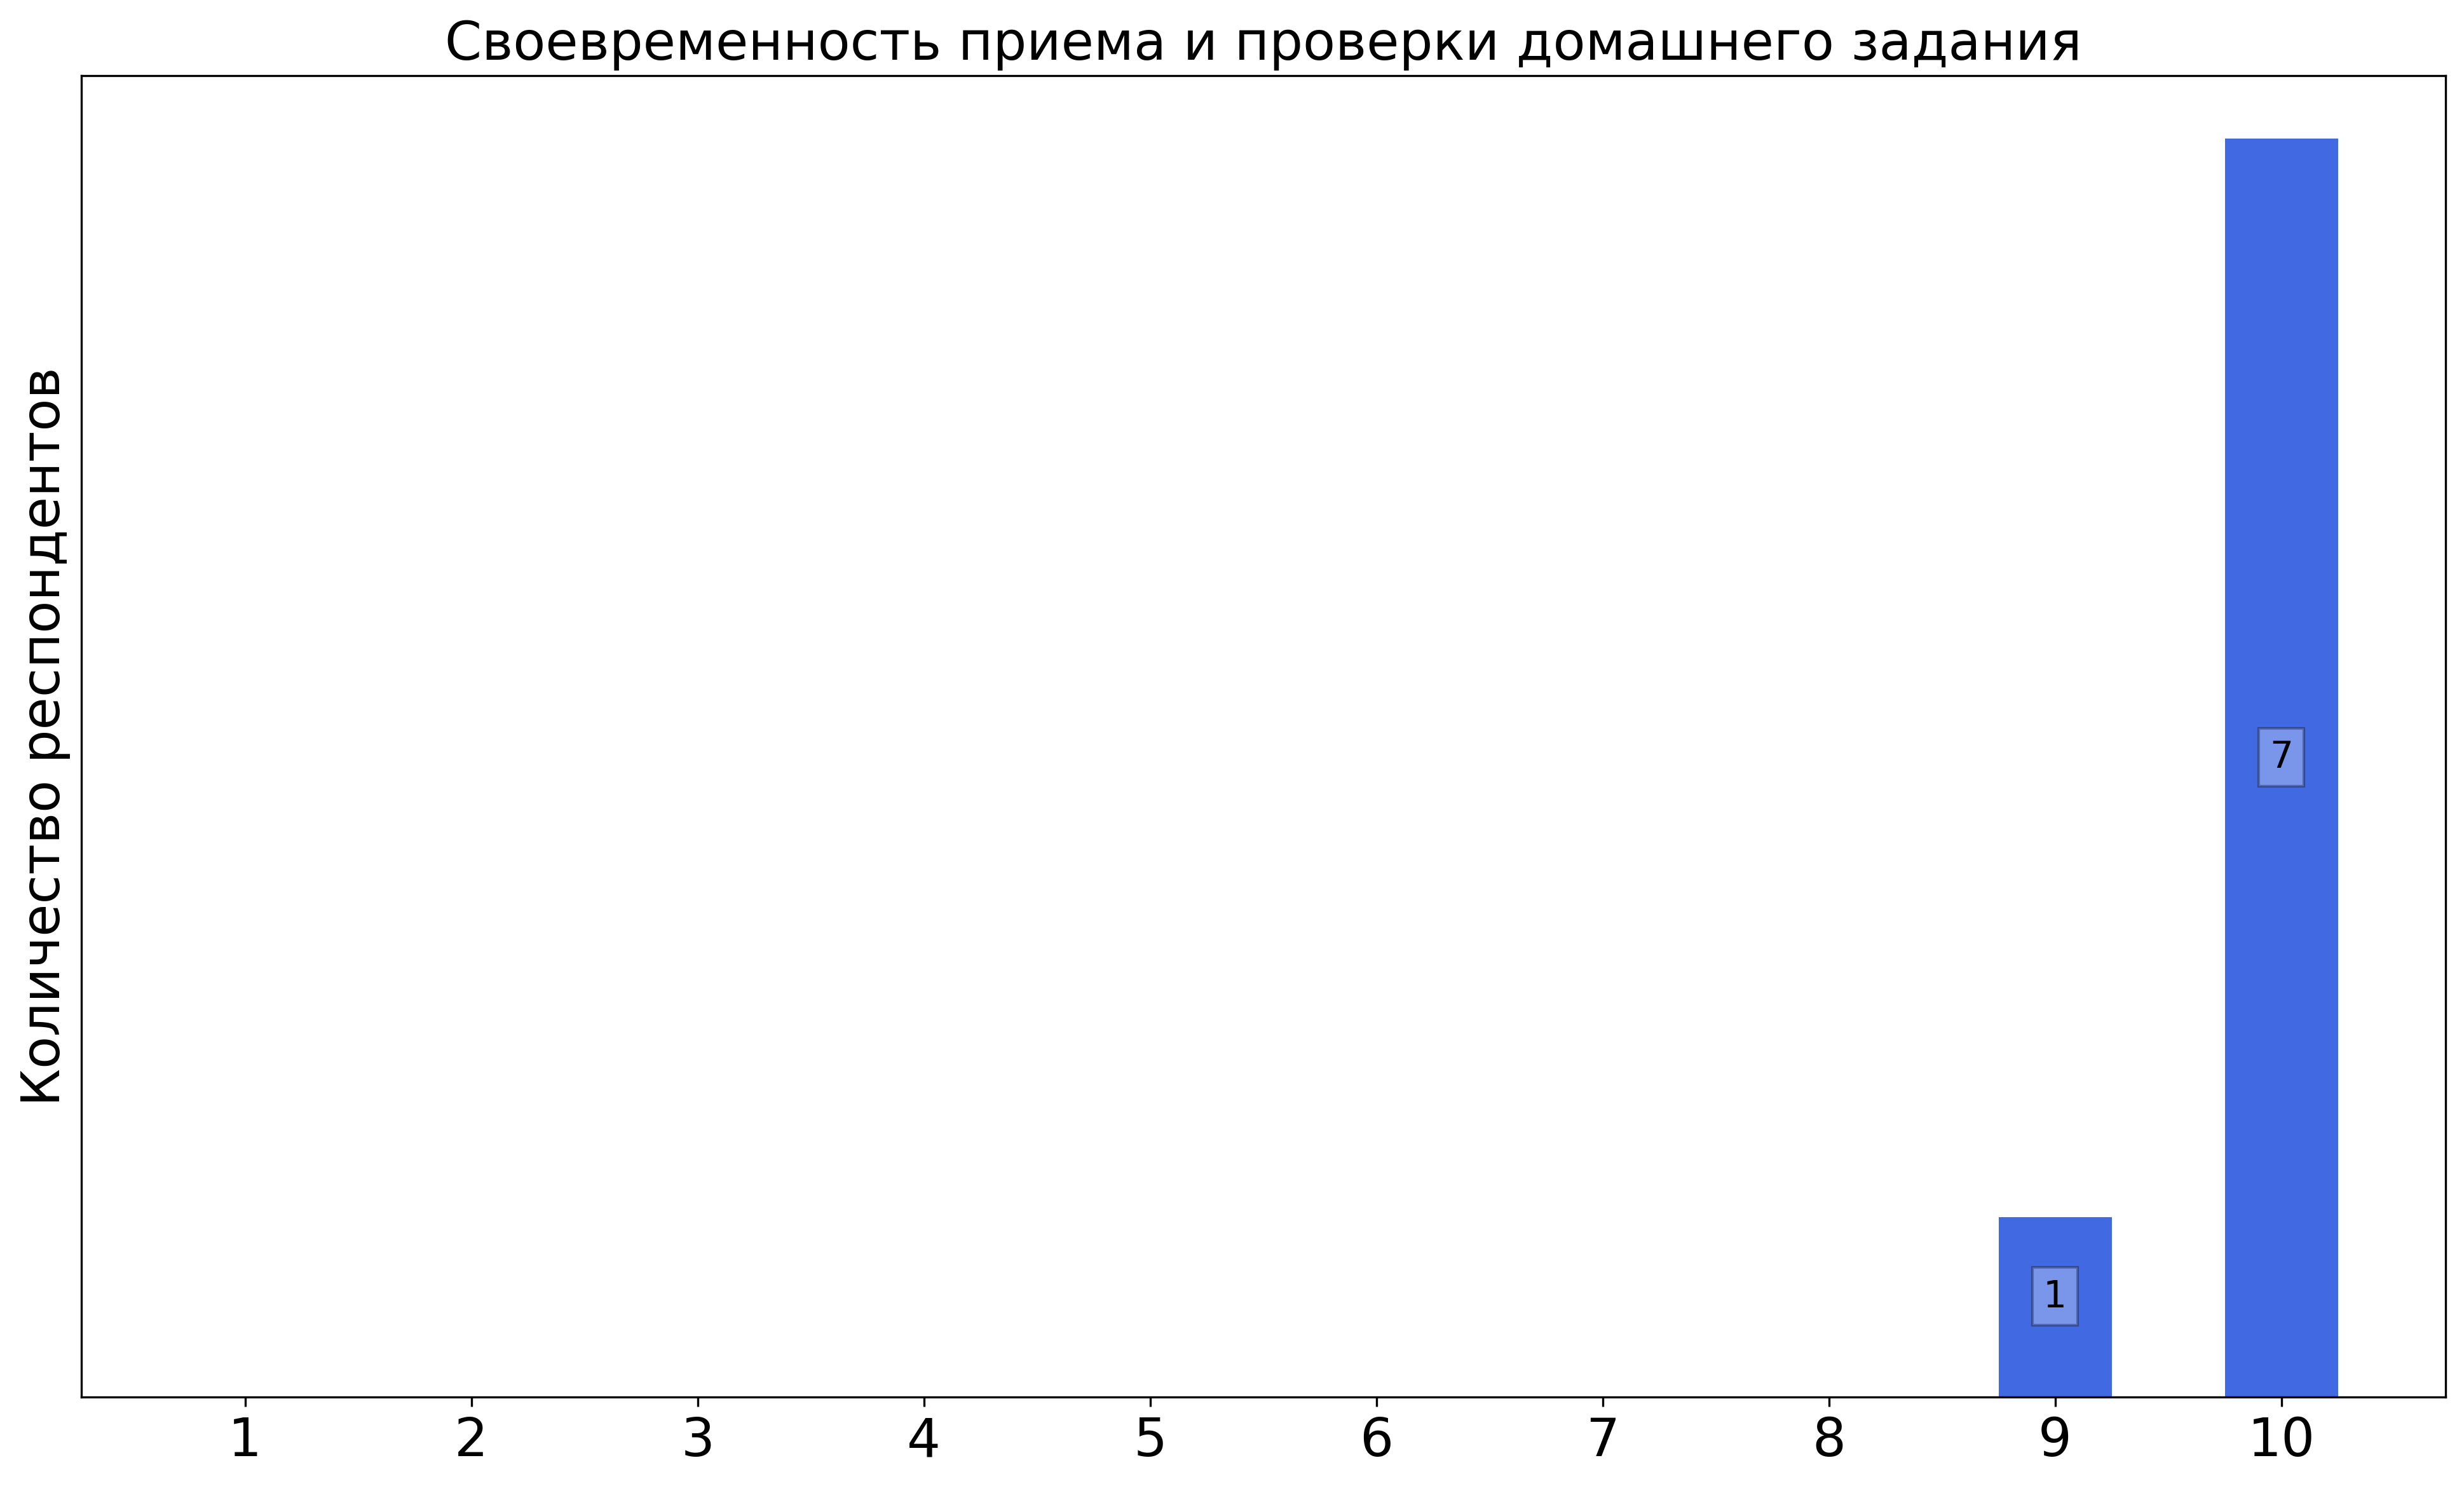
\includegraphics[width=\textwidth]{images/4 course/Введение в распараллеливание алгоритмов и программ/seminarists-marks-Лапушкин А.Г.-2.png}
			\end{subfigure}
			\begin{subfigure}[b]{0.45\textwidth}
				\centering
				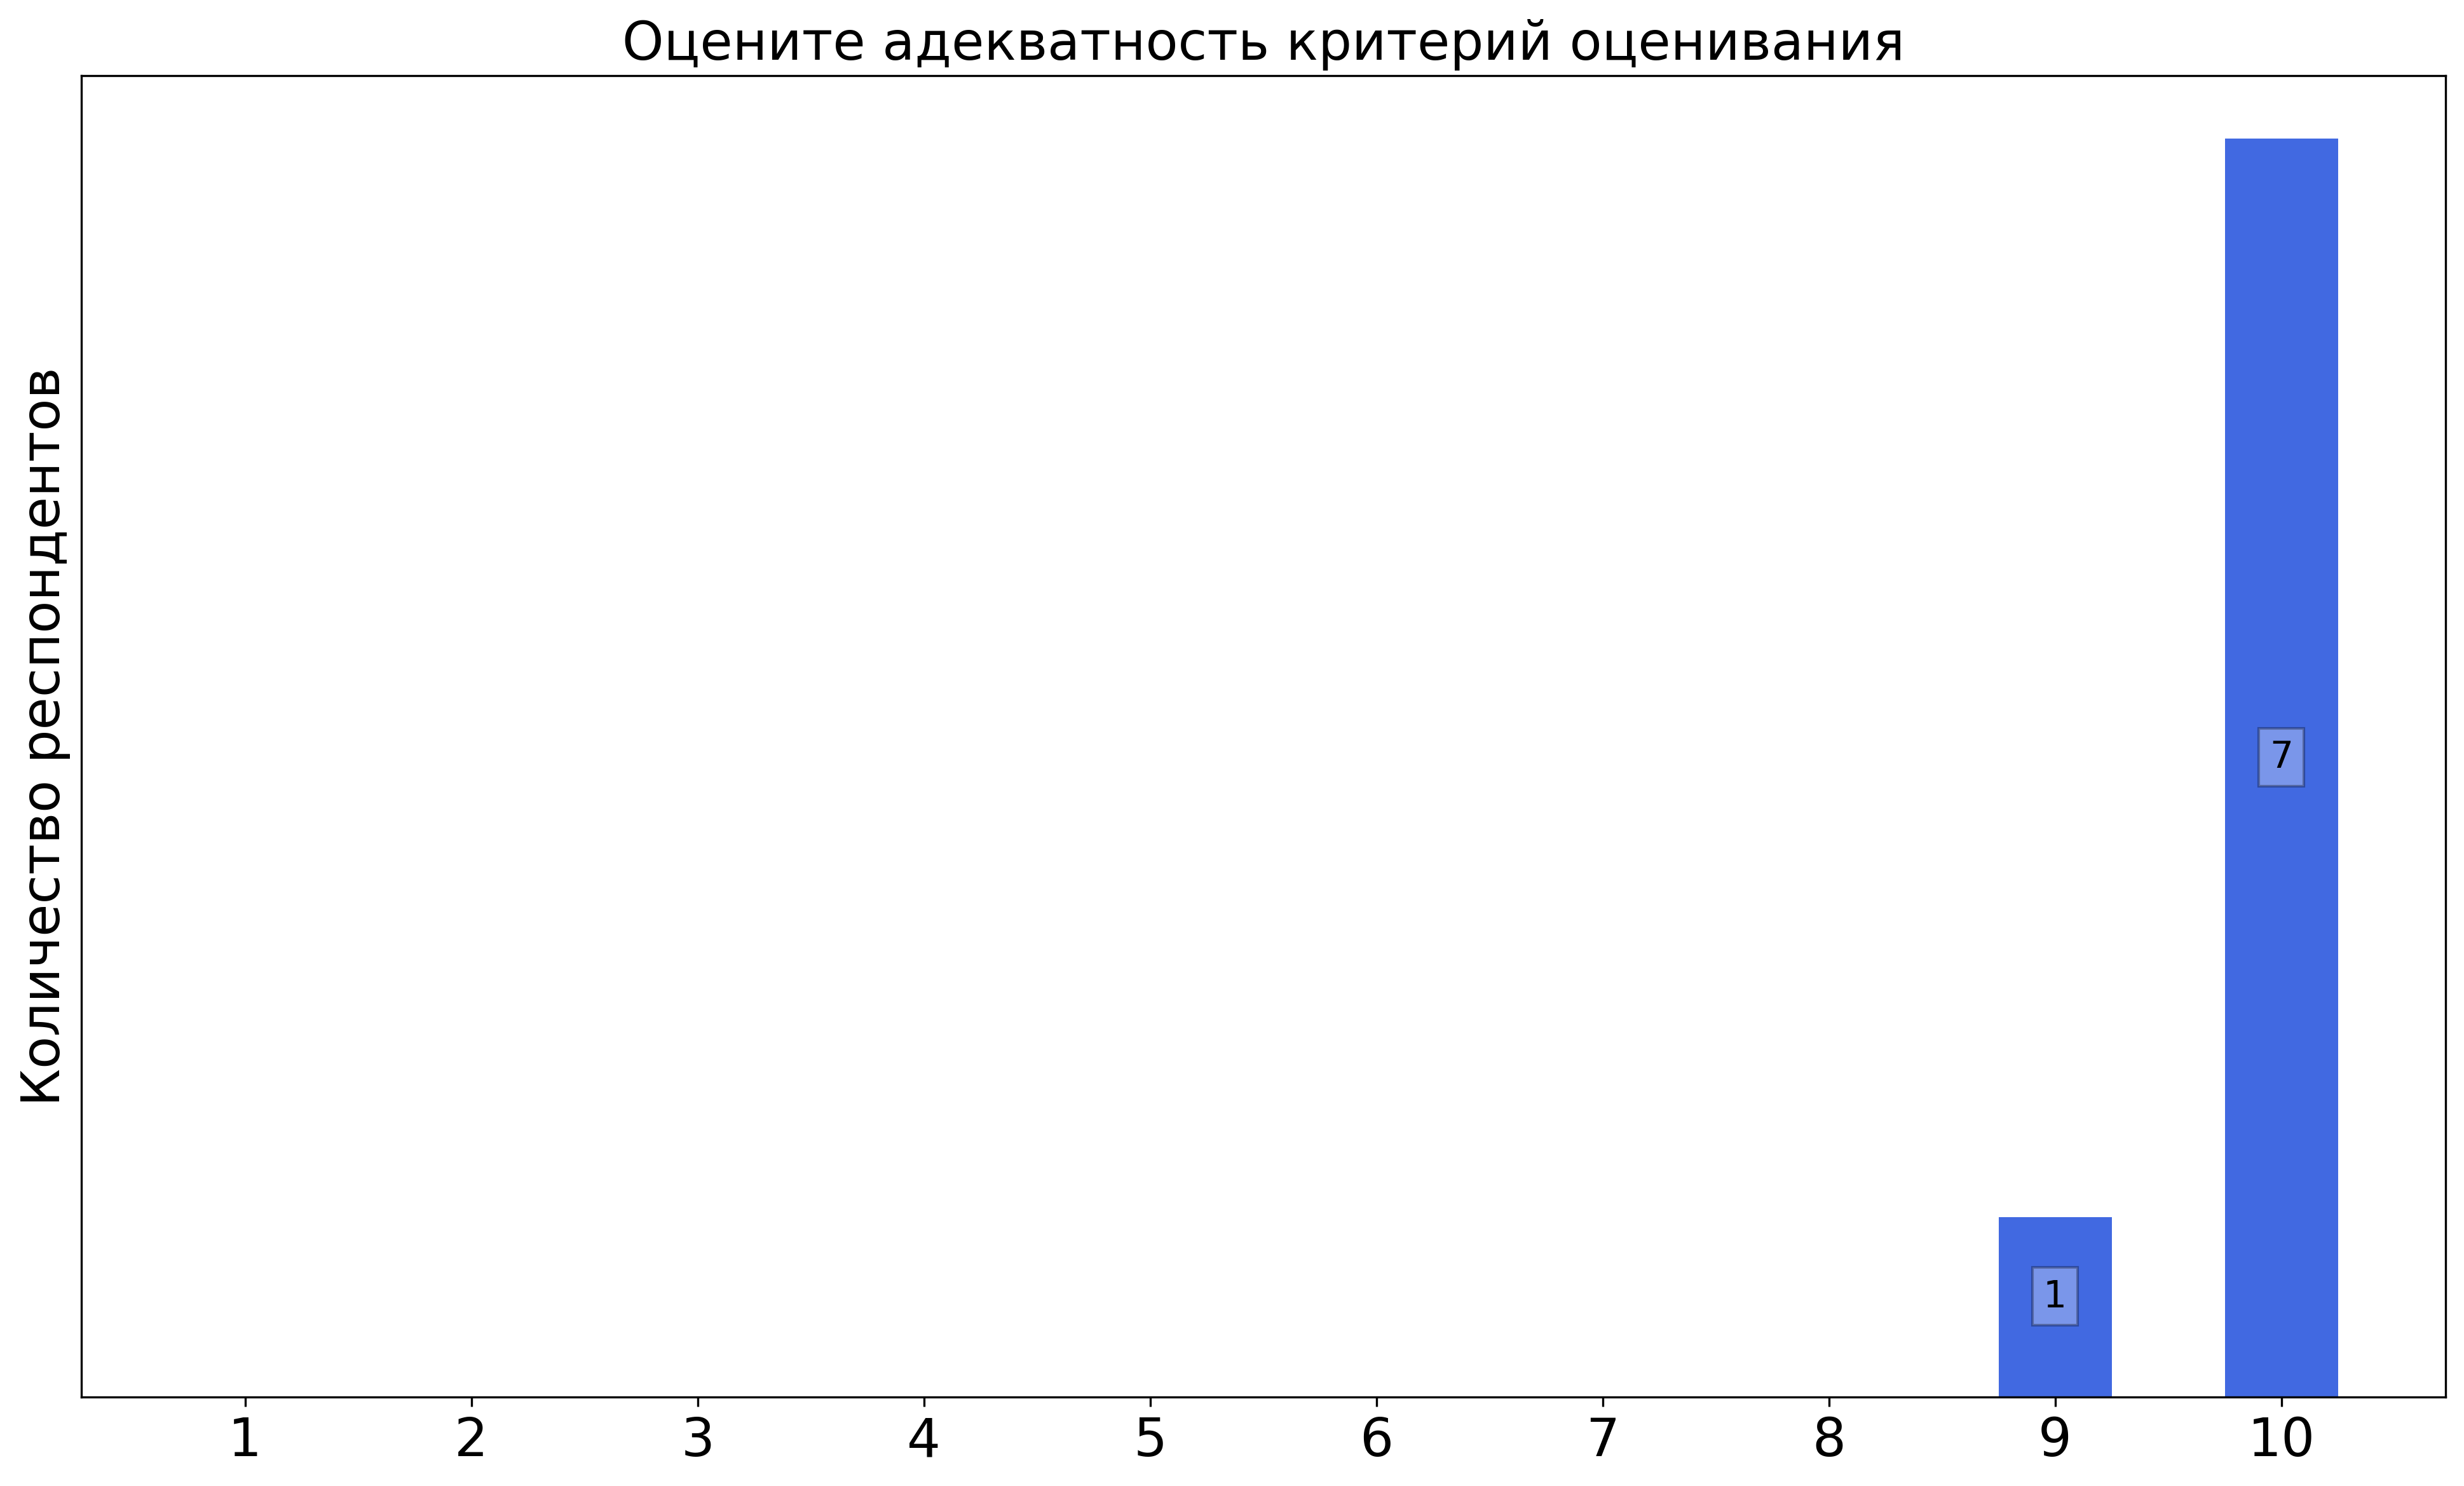
\includegraphics[width=\textwidth]{images/4 course/Введение в распараллеливание алгоритмов и программ/seminarists-marks-Лапушкин А.Г.-3.png}
			\end{subfigure}	
			\caption{Оценки респондентов о качестве преподавания семинаров}
		\end{figure}

		\textbf{Комментарии студентов о семинаристе\protect\footnote{сохранены оригинальные орфография и пунктуация}}
            \begin{commentbox} 
                Отличный семинарист, на занятиях рассказывает гораздо больше теоретических вещей, понятно объясняет. 
            \end{commentbox} 
        
            \begin{commentbox} 
                Невероятный. Курс держится на нём для меня. Объясняет потрясающе, готовится  семинарам, интересуется темой и в своё свободное время и приносит дополнительные материалы помимо основной программы курса.
        
                Объясняет понятно, разжёвывает даже моменты напрямую не касающиеся темы. Показывает примеры в коде. Сам составляет шикарные информативные презентации. 
        
                Выкладывает домашки и обговаривает срок. Всегда готов их принять.  
            \end{commentbox} 


    \subsubsection{Отзыв студентов о семинарах. Семинарист: Пальян Р.Л.}
        \begin{figure}[H]
            \centering
            \begin{subfigure}[b]{0.45\textwidth}
                \centering
                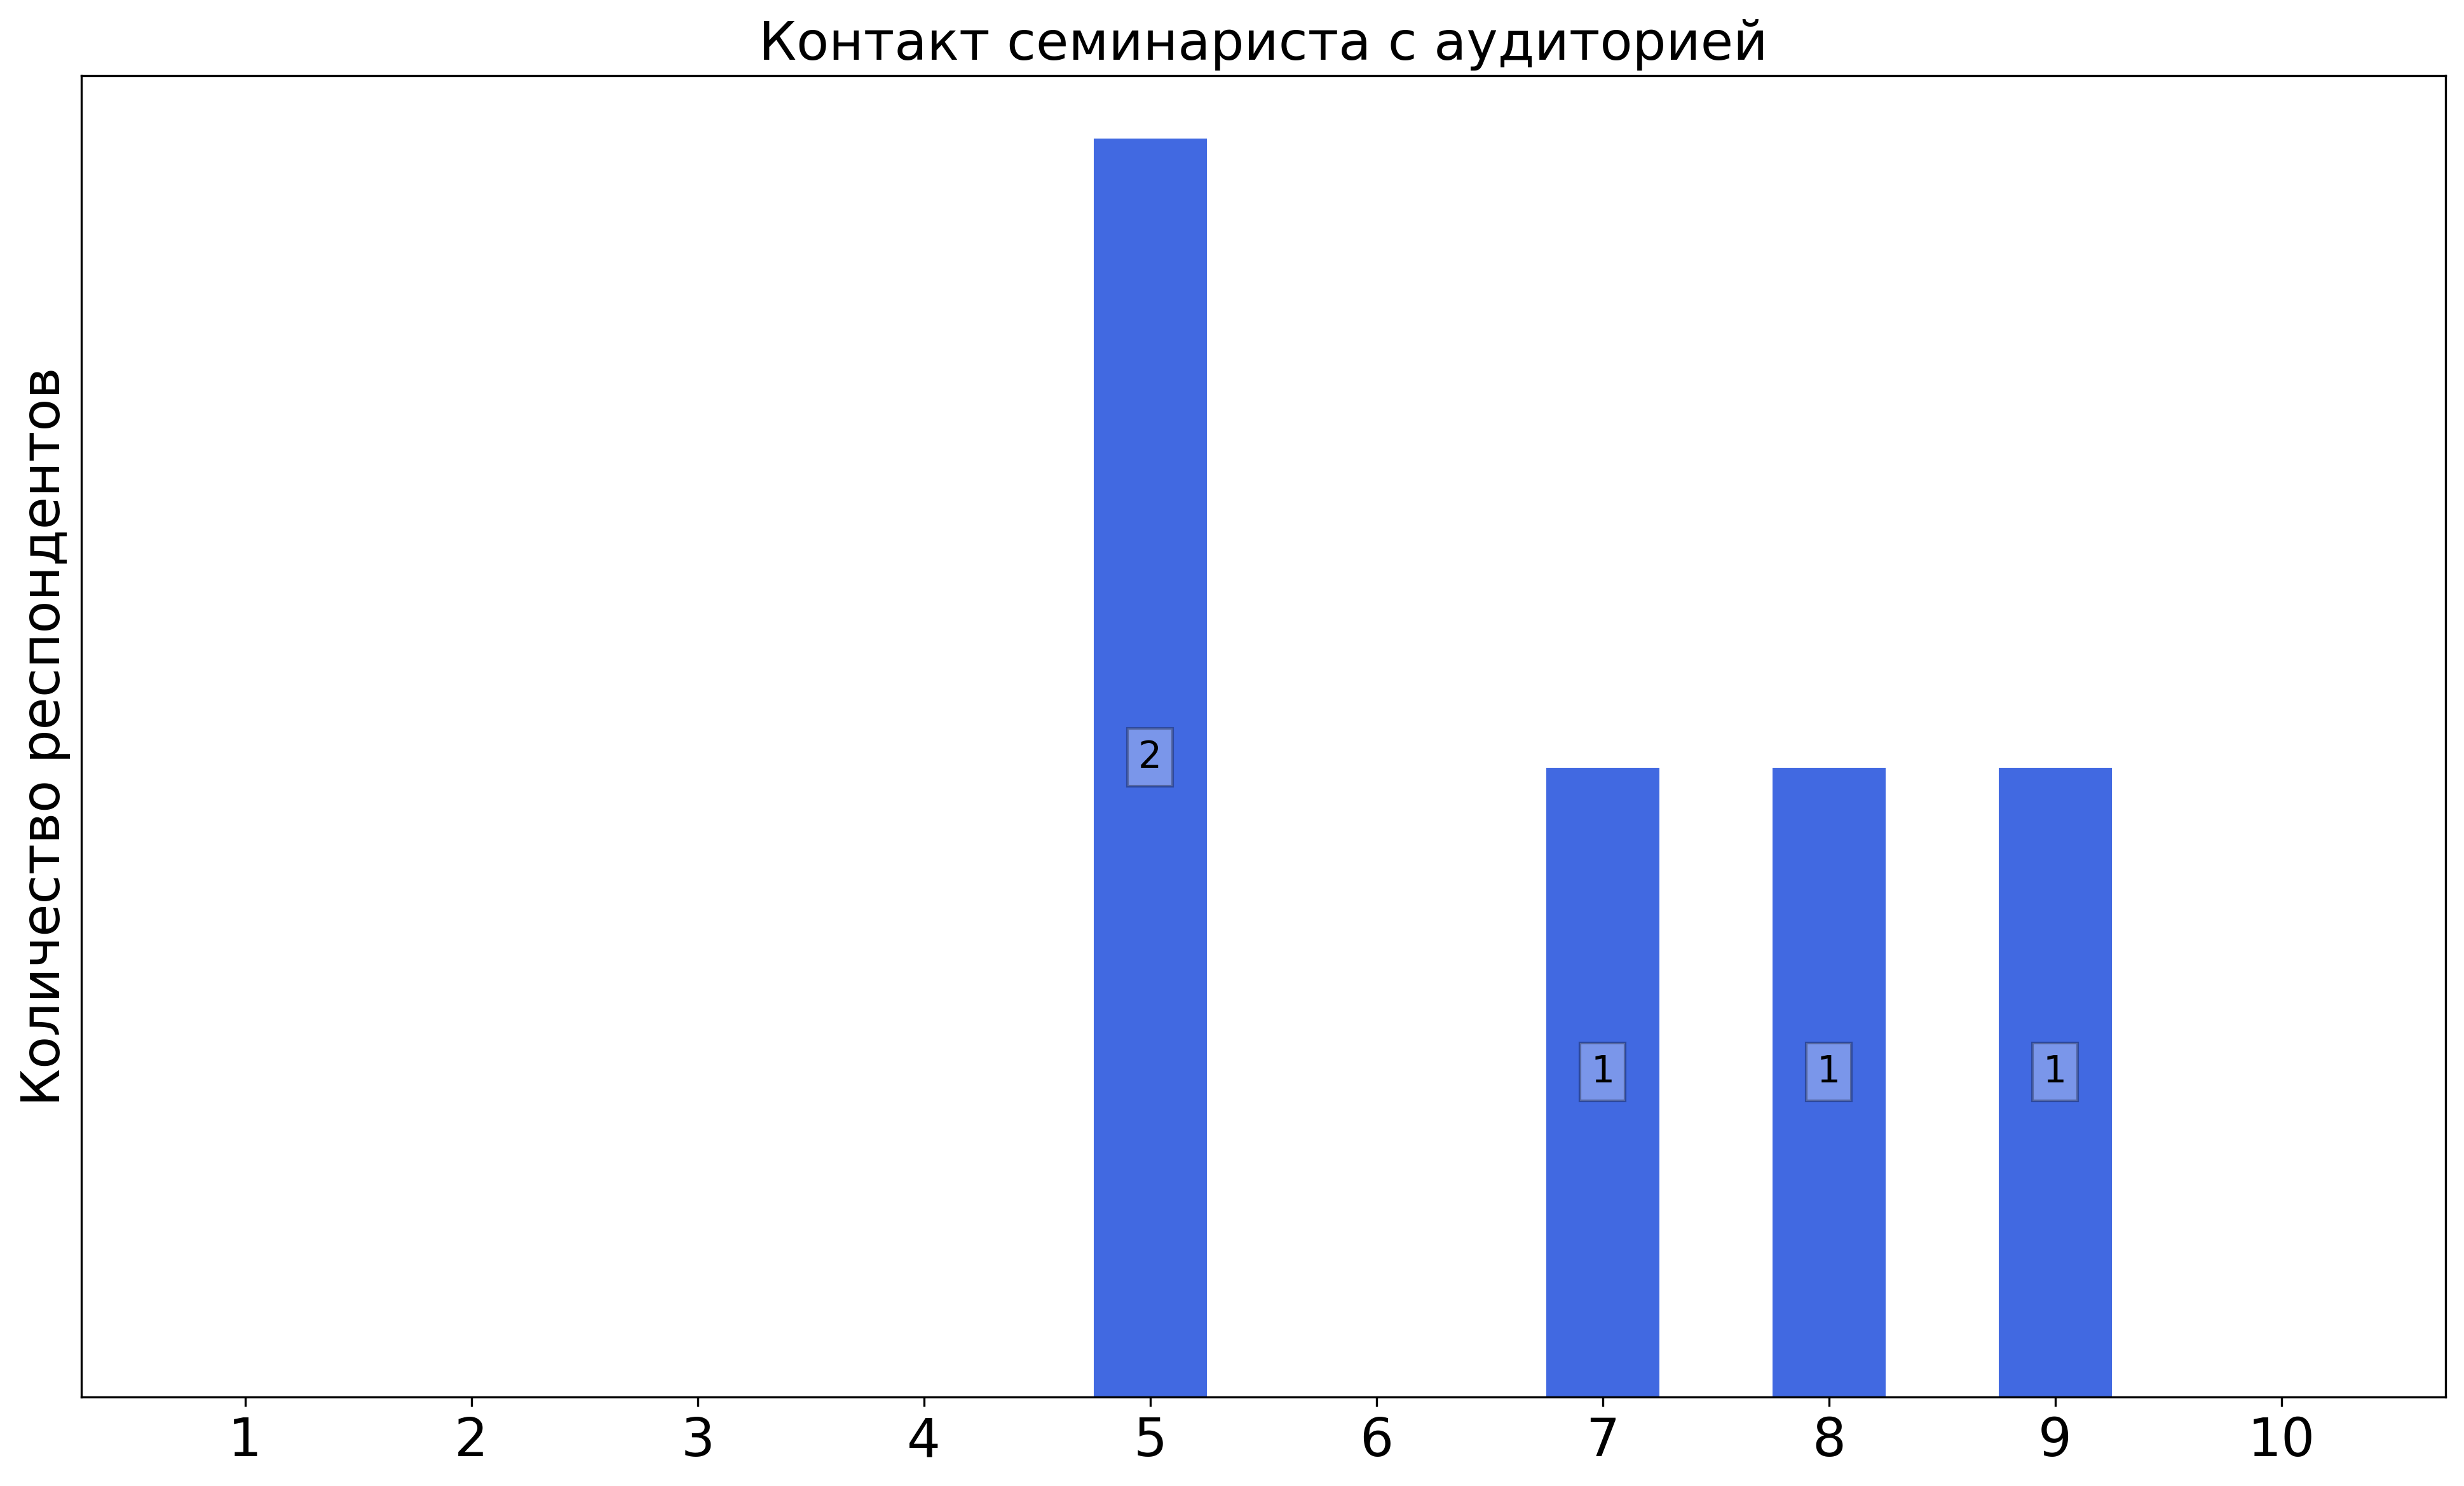
\includegraphics[width=\textwidth]{images/4 course/Введение в распараллеливание алгоритмов и программ/seminarists-marks-Пальян Р.Л.-0.png}
            \end{subfigure}
            \begin{subfigure}[b]{0.45\textwidth}
                \centering
                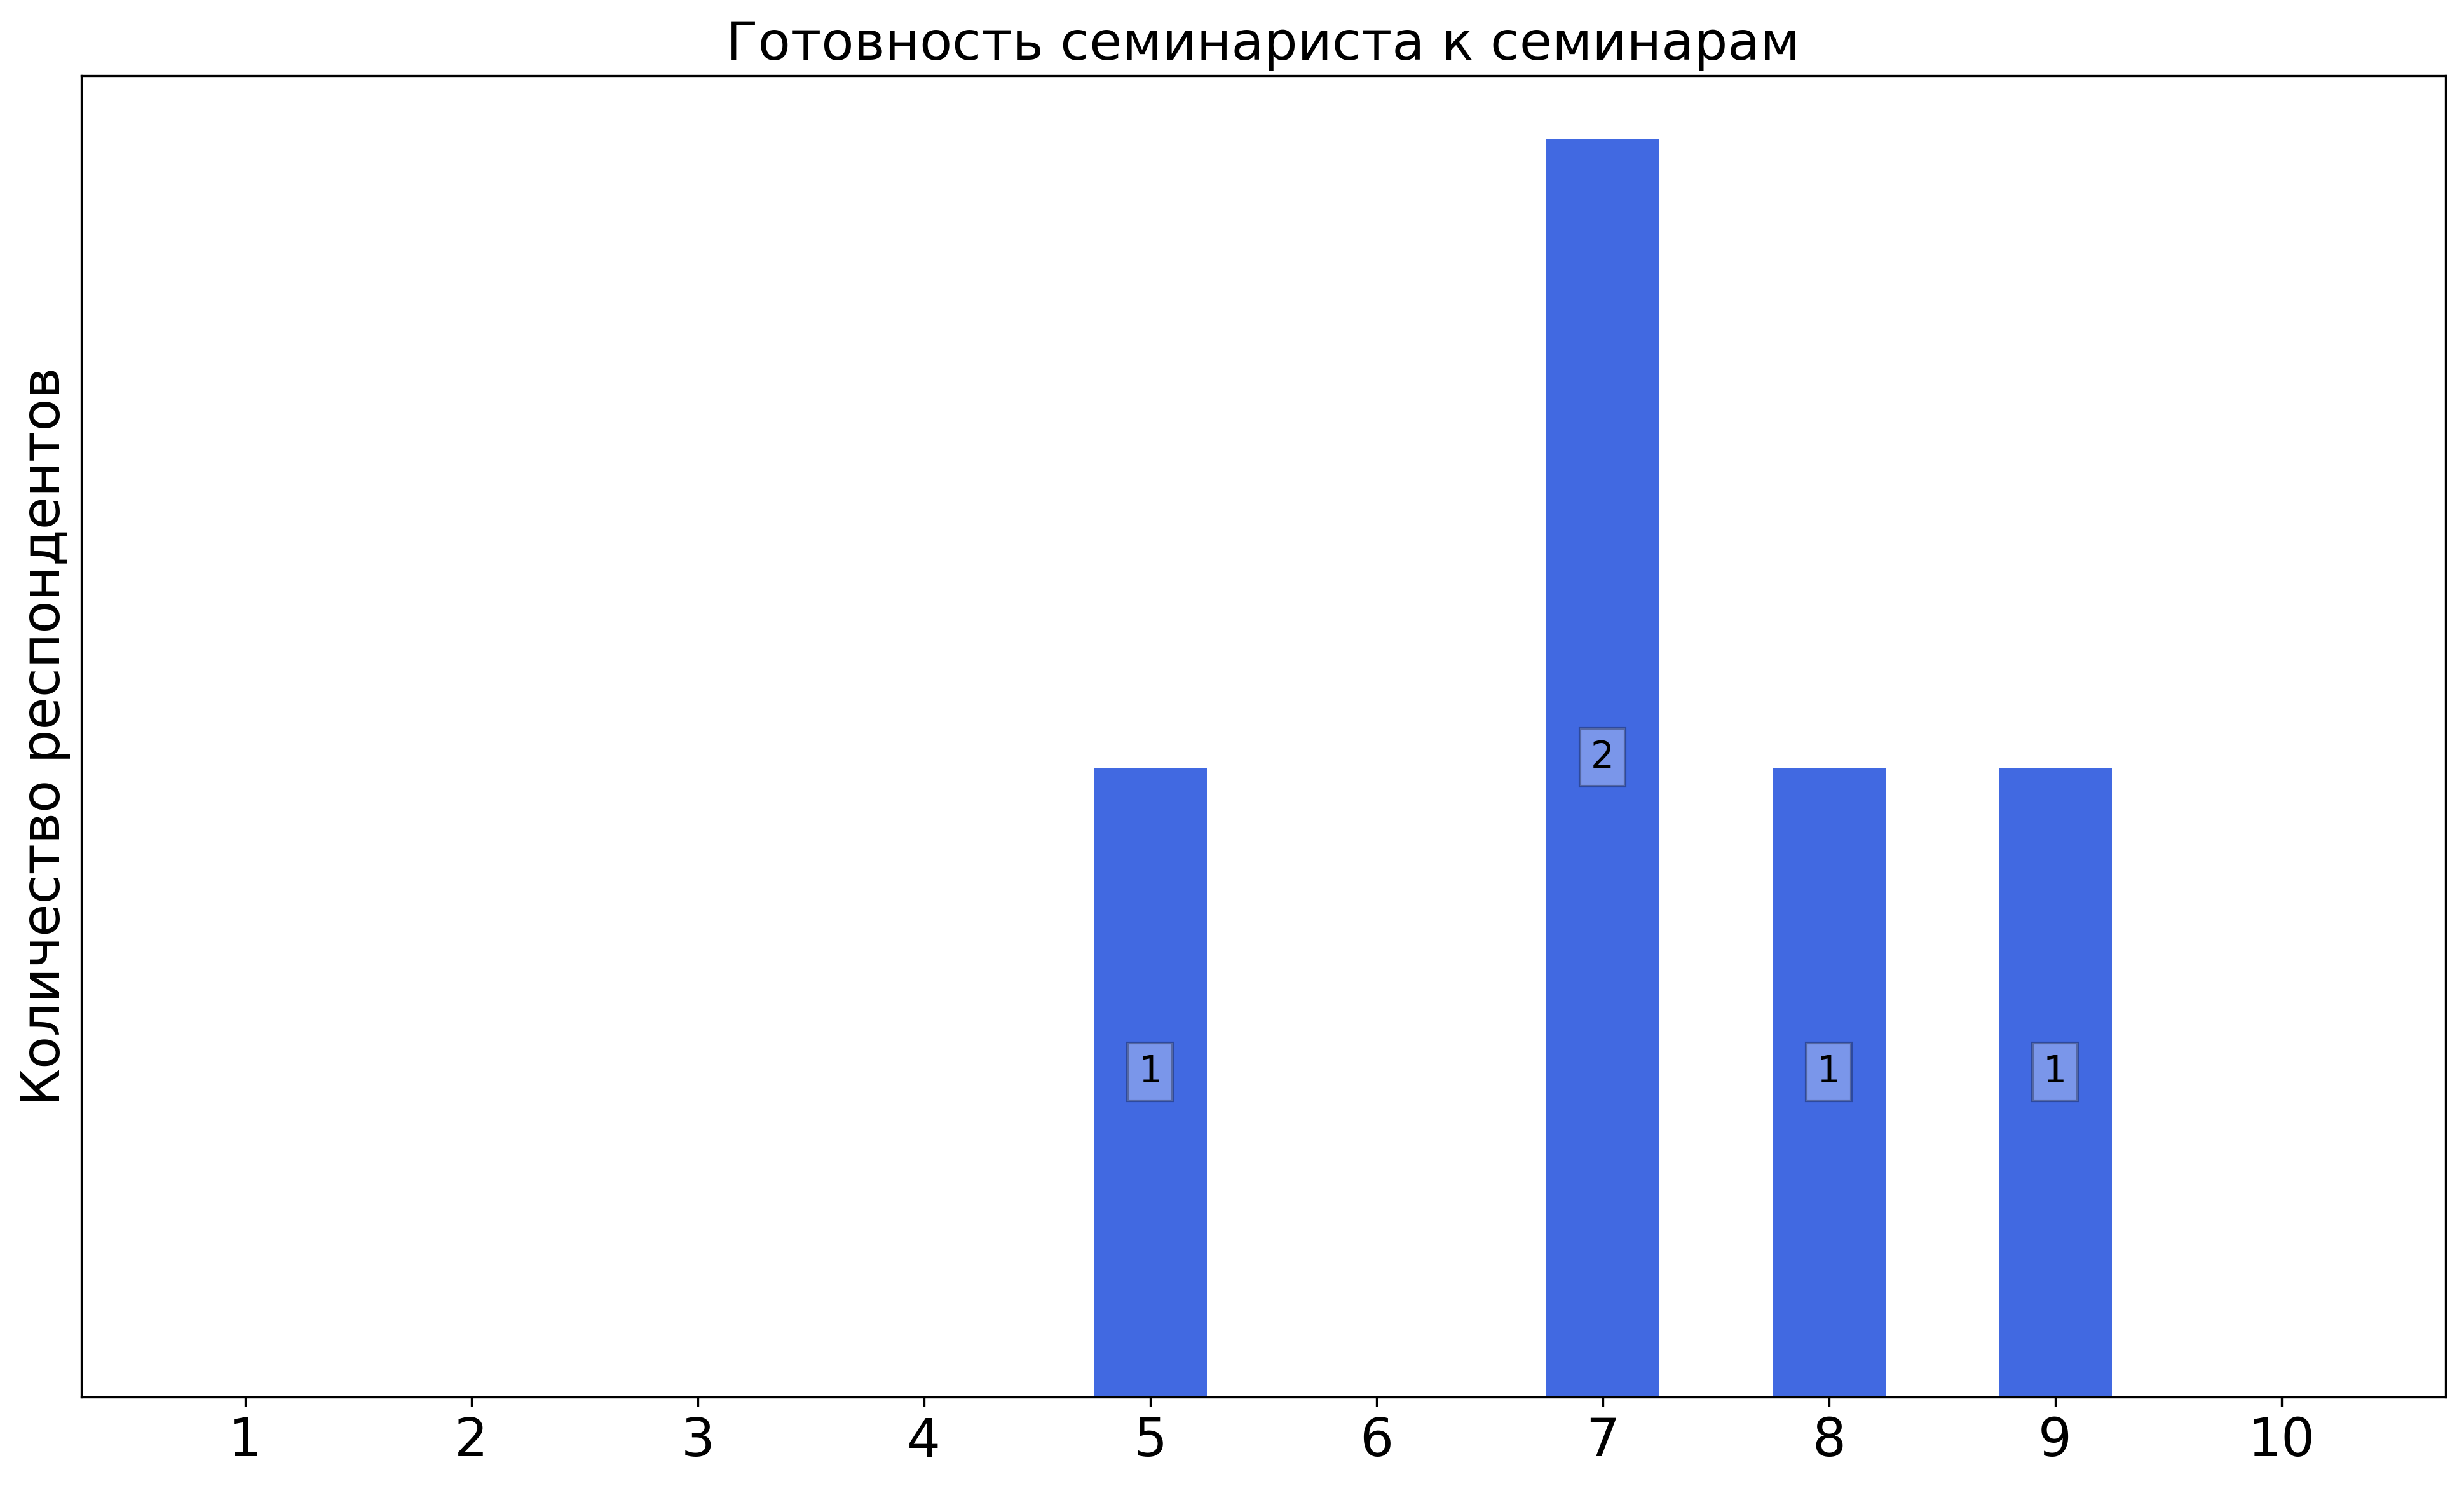
\includegraphics[width=\textwidth]{images/4 course/Введение в распараллеливание алгоритмов и программ/seminarists-marks-Пальян Р.Л.-1.png}
            \end{subfigure}
            \begin{subfigure}[b]{0.45\textwidth}
                \centering
                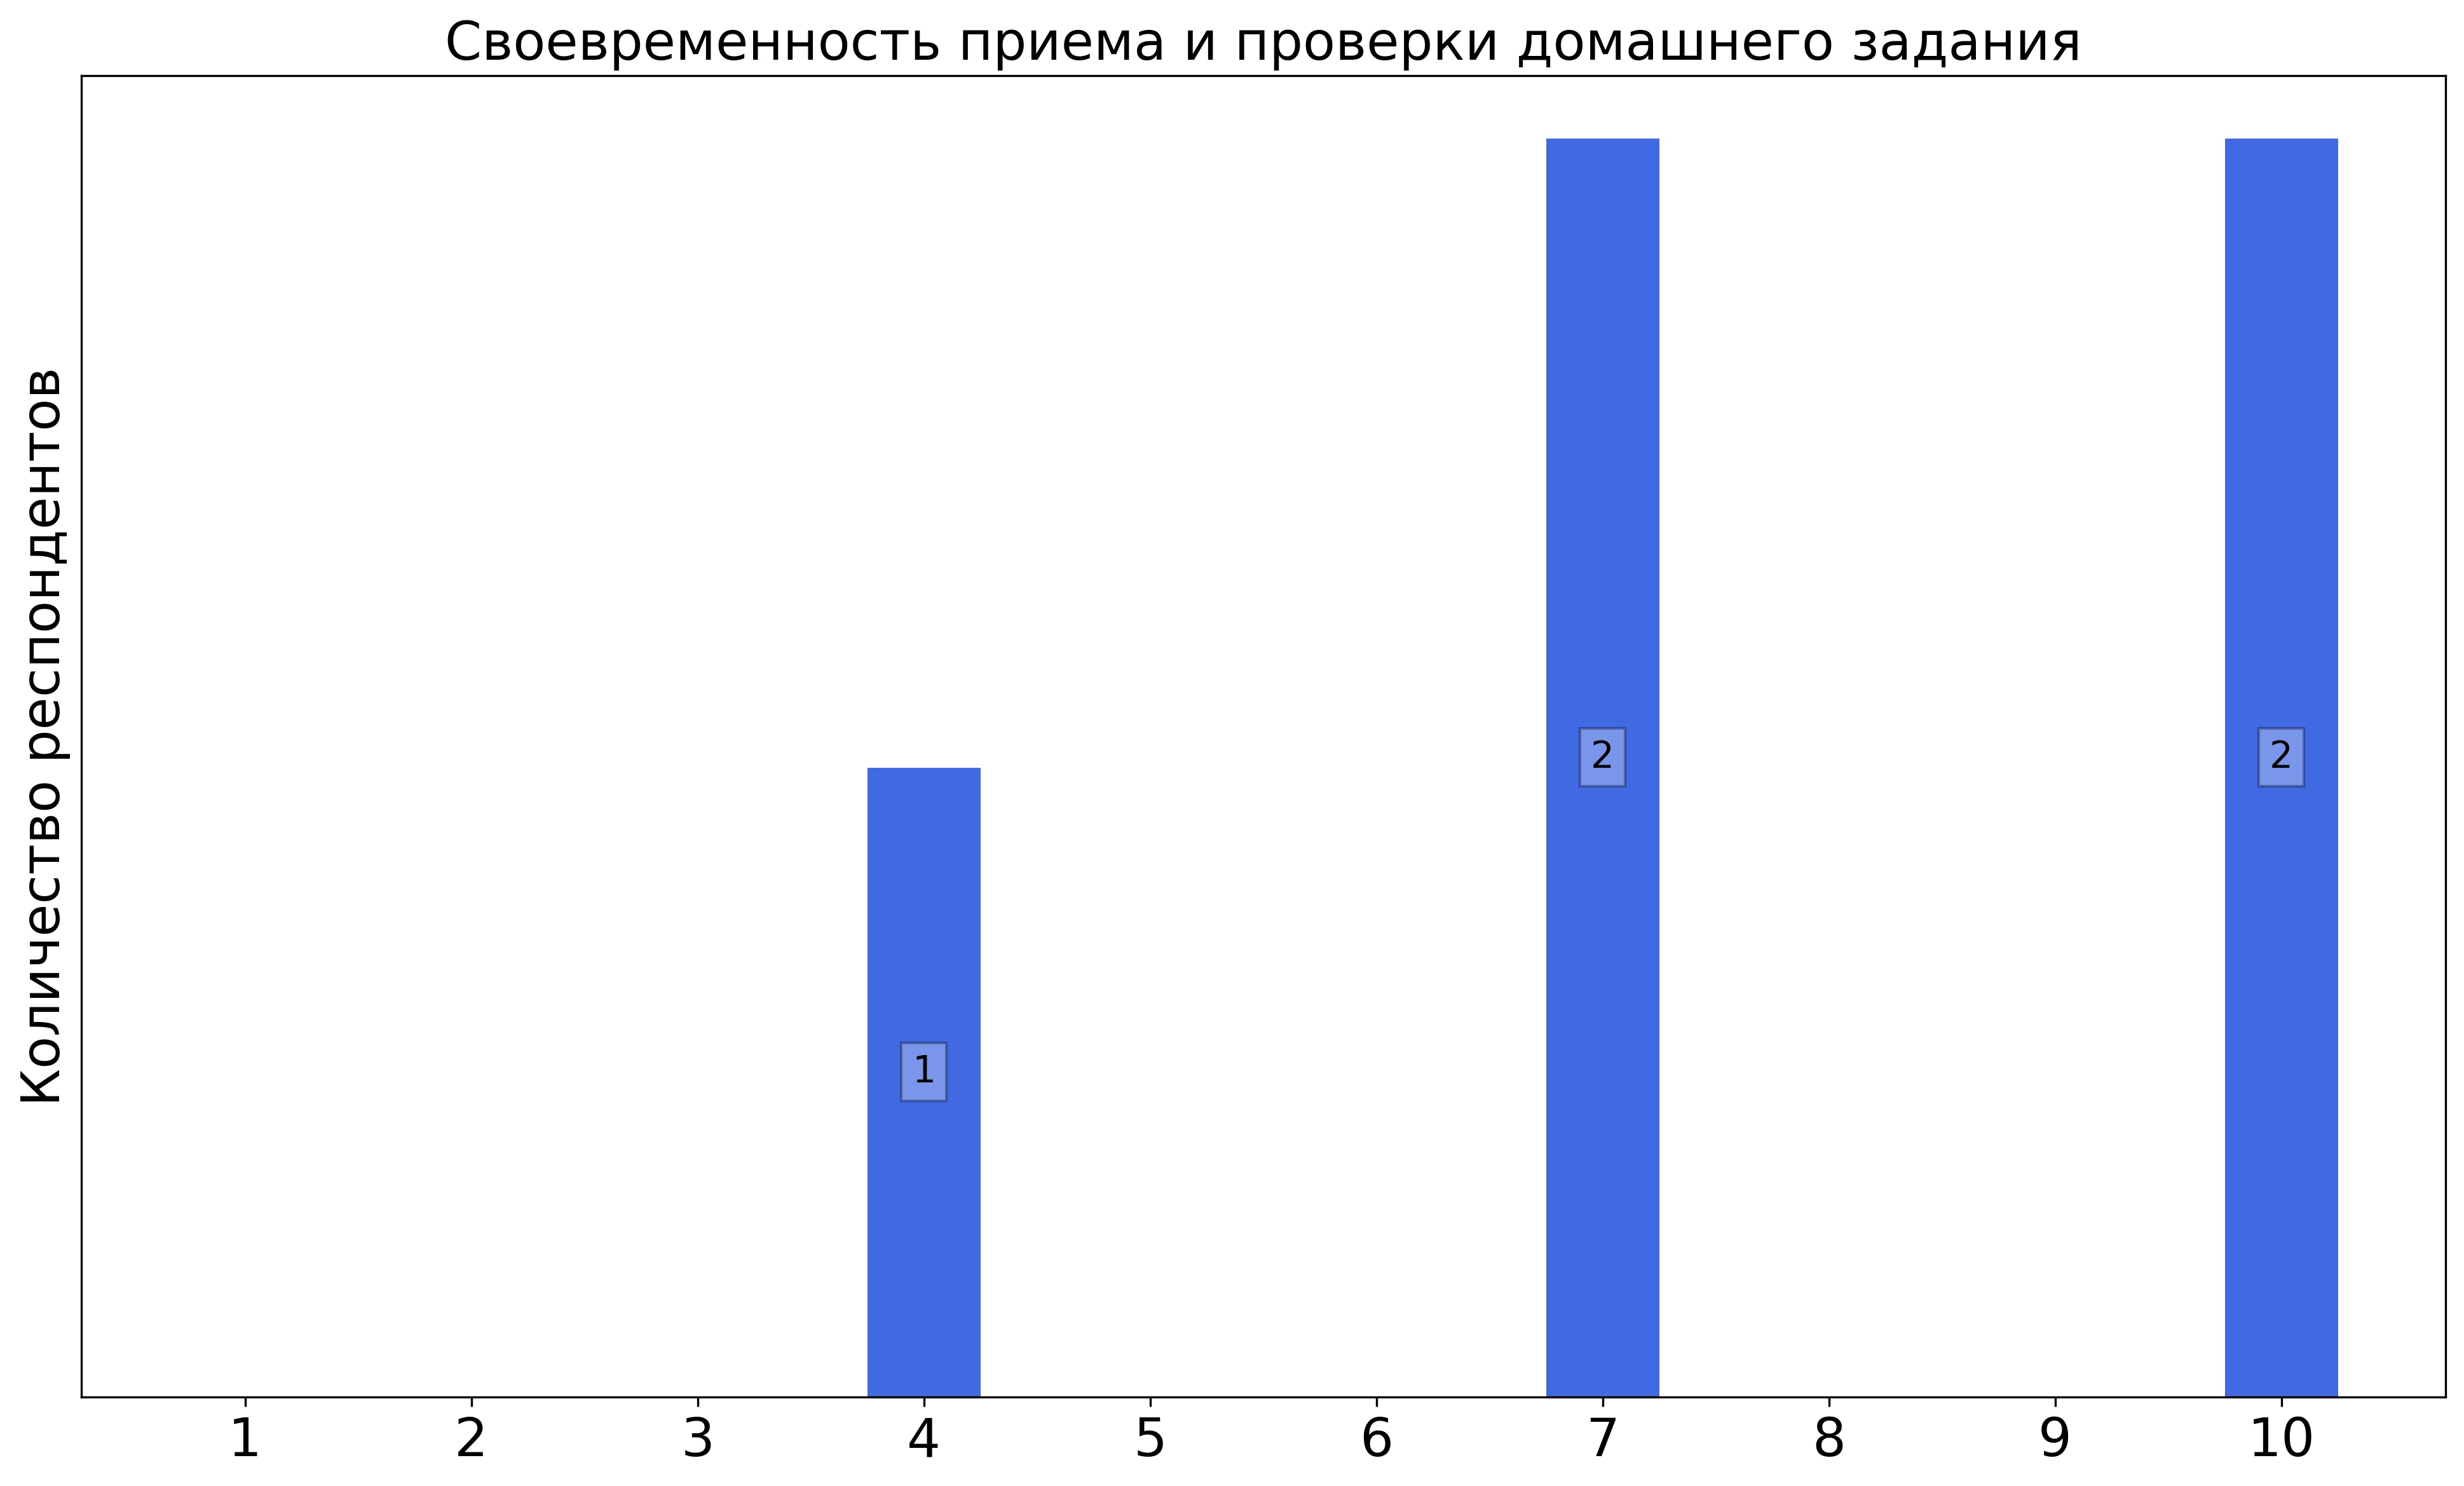
\includegraphics[width=\textwidth]{images/4 course/Введение в распараллеливание алгоритмов и программ/seminarists-marks-Пальян Р.Л.-2.png}
            \end{subfigure}
            \begin{subfigure}[b]{0.45\textwidth}
                \centering
                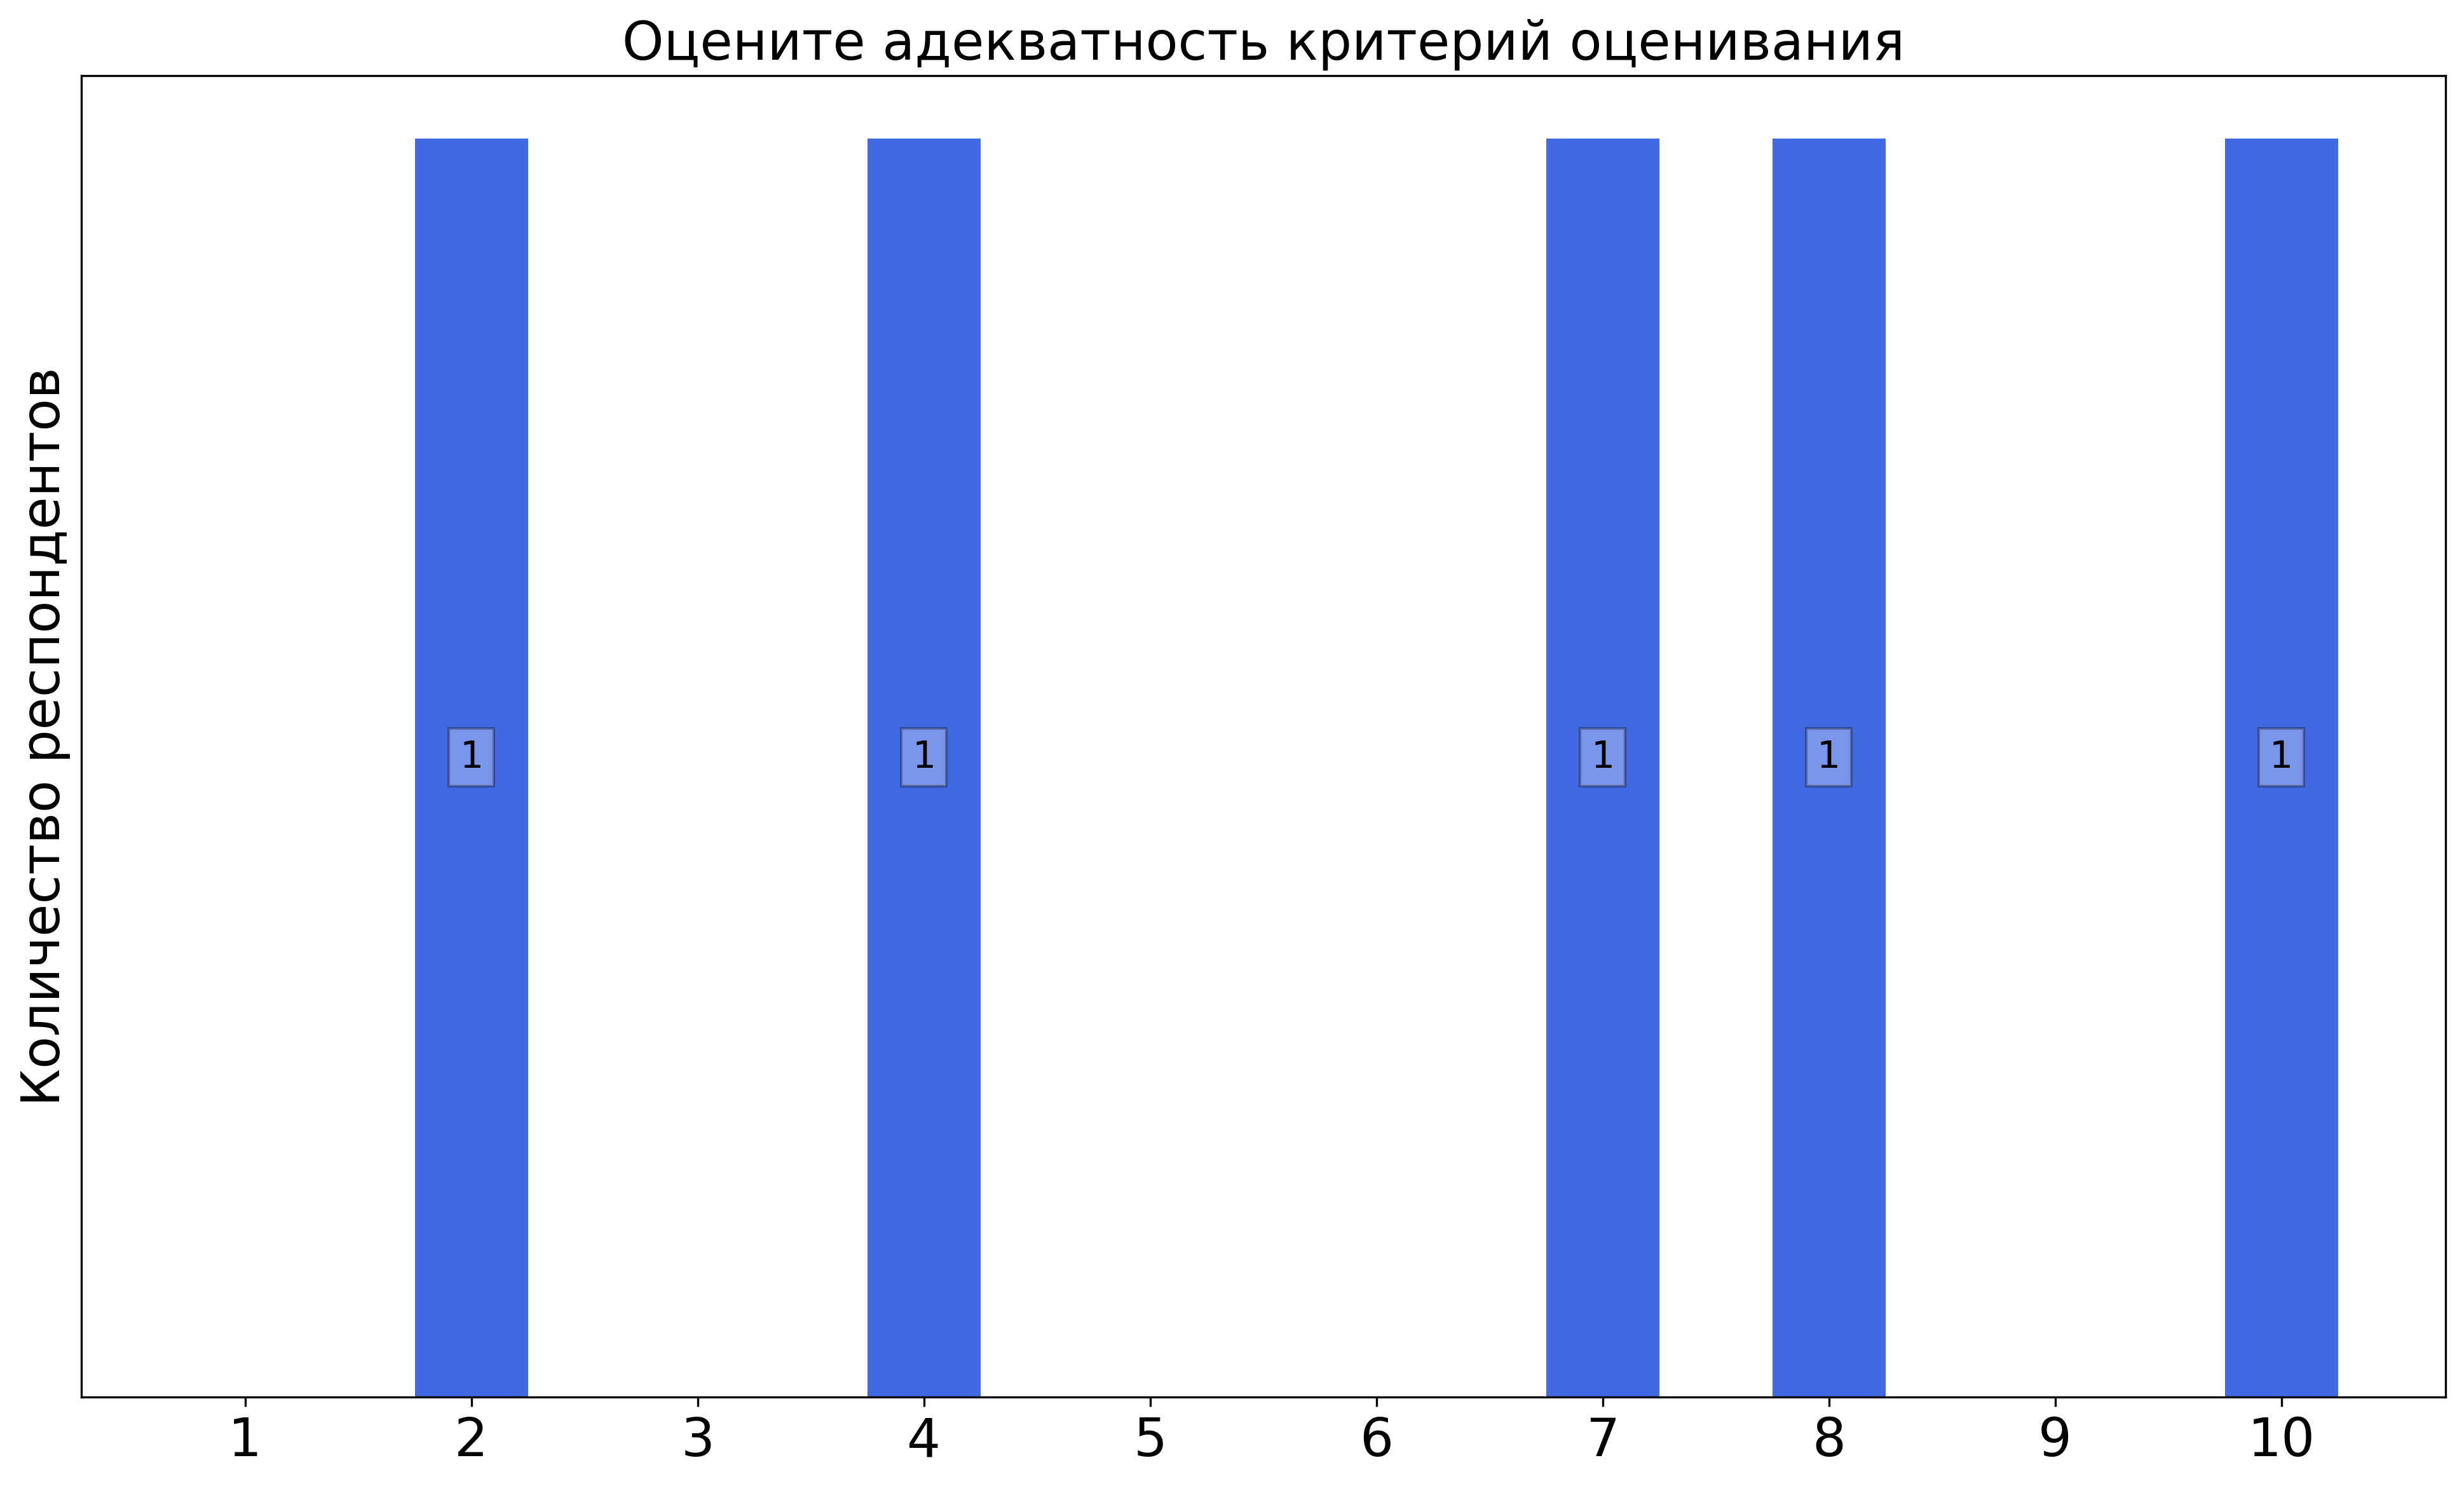
\includegraphics[width=\textwidth]{images/4 course/Введение в распараллеливание алгоритмов и программ/seminarists-marks-Пальян Р.Л.-3.png}
            \end{subfigure}	
            \caption{Оценки респондентов о качестве преподавания семинаров}
        \end{figure}

        \textbf{Комментарии студентов о семинаристе\protect\footnote{сохранены оригинальные орфография и пунктуация}}
            \begin{commentbox} 
                Семинарист очень лояльный. Можно не посещать и сдать все в конце семестра, но если ходить на семинары то что рассказывает в большинстве своем не очень интересно и современно. Однако как специалист он если его специально спросить по какой то теме которая может даже не связана с распараллеливанием но связана с программированием, тогда он хорошо и интересно рассказывал. Идет на встречу студентам, тк я в большой группе не все успевали сдать задачи и он задерживался на пару часов ради того чтобы все сдали. На семинары мало кто ходил, он за это не обижался.  
            \end{commentbox} 
        
            \begin{commentbox} 
                Душно((( 
            \end{commentbox} 
        
            \begin{commentbox} 
                Странно, что задание он принимает по принципу, кто больше ходил на занятия, тот первый сдает. Всё неплохо звучит на первый взгляд, но проблема в том, что он "отличникам" даёт доп задания условно с 9 на 10 поднять, в начале сдачи их долго обсуждает, потом на некоторых не хватает времени, им приходится приходить в другой раз даже не приступив к сдаче. На следующей сдаче они опять оказываются в конце очереди и могут вновь не иметь возможности приступить к сдаче, даже чтобы сдать просто на хоть какую-нибудь оценку. 
            \end{commentbox}
    
    \subsubsection{Прочие комментарии и предложения по улучшению курса}
            \begin{commentbox}
                Хотелось бы видеть более современные фреймворки и более интересные задания семинарские. У нашего семинариста были базовые очень простые задачки и две лабы + кр. + доп задачки и в целом расчитывалось что доп задачи это как раз и даст всю интересность. Но увы времени на это не хватило.
            \end{commentbox}

            \begin{commentbox}
                В нынешнем виде курс бесполезен, заисключнием семинаров Лапушкина. Возможно следует построить курс по его презентациям или подсмотреть аналогичный курс на фпми от Липовского, который в несколько раз полезнее и интереснее
            \end{commentbox}

            \begin{commentbox}
                Курс работает  за счет семинаров. 2й семестр на лекциях чем-то похож на вычматы (судя по контрольной)
            \end{commentbox}

            \begin{commentbox}
                Многие концепции устарели, было бы интересно узнать и о каких-то более новых возможностях, возможно, как это сейчас делается в языках типо go, rust, в современных веб-серверах, или, наоборот, на более низком уровне.
            \end{commentbox}